\documentclass[spanish,12pt,a4paper,final,oneside]{book}
\setlength{\headheight}{14pt}
\setlength{\parindent}{0pt}
\setlength{\parskip}{0.5em}
\usepackage[spanish]{babel}
\usepackage[utf8]{inputenc}
\usepackage[bottom]{footmisc}
\usepackage[a4paper, total={15cm, 24cm}]{geometry}

\addtolength{\skip\footins}{2pc plus 5pt}

\usepackage{enumitem}
\setlist{topsep=0pt}

\usepackage{longtable}
\setlength{\tabcolsep}{12pt}

\usepackage{amsmath}
\usepackage{amsfonts}
\usepackage{amssymb}

\usepackage{graphicx}
\graphicspath{ {./imagenes/} }

\usepackage{listings}
\usepackage{courier}
\usepackage{xcolor}
\lstset{
    basicstyle=\footnotesize\ttfamily,
    commentstyle=\color{lightgray},
    stringstyle=\color{brown},
    % keywordstyle=\color{orange},
    % backgroundcolor=\color{lime},
    breaklines=true,   % Lines will be wrapped
    frame=b,
    % numbers=left,
    numberstyle=\tiny\color{lightgray},
    numbersep=5pt,
    extendedchars=true,
    showspaces=false,
    showtabs=false,
    showstringspaces=false,
    tabsize=2,
    xleftmargin=17pt,
    framexleftmargin=17pt,
    framexrightmargin=5pt,
    framexbottommargin=4pt,
    literate=
      {ñ}{{\~n}}1
      {Ñ}{{\~N}}1
      {¿}{{?'}}1
      {¡}{{!'}}1
      {á}{{\'a}}1
      {Á}{{\'A}}1
      {é}{{\'e}}1
      {É}{{\'E}}1
      {í}{{\'i}}1
      {Í}{{\'I}}1
      {ó}{{\'o}}1
      {Ó}{{\'O}}1
      {ú}{{\'u}}1
      {Ú}{{\'U}}1
      {â}{{\^a}}1
      {€}{{\euro}}1
}
\lstloadlanguages{ % Check documentation for further languages ...
     Java,
     C++,
     Python,
     XML
}
\usepackage{caption}
\DeclareCaptionFont{white}{\color{white}}
\DeclareCaptionFormat{listing}{\colorbox[cmyk]{0.43, 0.35, 0.35,0.01}{\parbox{\textwidth}{\vspace{15pt}#1#2#3}}}
\captionsetup[verbatim]{format=listing,labelfont=white,textfont=white, singlelinecheck=false, margin=0pt, font={bf,footnotesize}}

\usepackage[colorlinks]{hyperref}
\hypersetup{colorlinks=true}
\hypersetup{urlcolor=blue}
\usepackage{cleveref}

\usepackage{fancyhdr}
\fancyhf{}
\fancyhead[RE]{\small\scshape\nouppercase{\leftmark}}
\fancyhead[LO]{\small\scshape\nouppercase{\leftmark}}
\fancyhead[LE,RO]{\small\thepage}
\pagestyle{fancy}

\usepackage{authoraftertitle}
\title{Más allá del IF y del WHILE}
\author{Juan Murua Olalde}
\date{19/Julio/2020}


\begin{document}

\begin{titlepage}

\begin{flushright}
\vspace{2cm}
\begin{Huge}\MyTitle\end{Huge}

Aprender a programar software\\ a base de ejercicios y ejemplos.
\\
\vspace{1cm}
\MyAuthor
\\
\vspace{1cm}
\MyDate
\\ \today
\\
\end{flushright}

\vfill
Nota: Una copia .pdf de este manual se puede descargar desde \url{www.susosise.es}
\\Nota: El código fuente y el historial de cambios de este documento se puede obtener en  \\ \url{https://github.com/JuanMuruaOlalde/DesarrolloDeSoftware}
\begin{flushleft}

\includegraphics[scale=0.3]{CreativeCommons-Attribution-ShareAlike-logo}
\begin{small}\url{https://creativecommons.org/licenses/by-sa/4.0}\end{small}
\end{flushleft}

\end{titlepage}

\hypersetup{linkcolor=black}
\tableofcontents


\chapter*{Requisitos previos}
Este libro asume que se está familiarizado y se tiene soltura manejando los aspectos básicos del lenguaje que se vaya a utilizar para realizar sus ejercicios.

Los aspectos que se dan por conocidos son:
\begin{itemize}
\item Un entorno sobre el que programar, con las herramientas básicas de: editor, compilador (o intérprete) y depurador.
\item Ejecución de programas, cuál es el punto de arranque (main).
\item Depuración de programas, cómo colocar puntos de interrupción (breakpoints) y cómo seguir el programa paso a paso visualizando valores en las variables escogidas.
\item Declaración de variables para almacenar distintos tipos de datos. Asignación de valores a variables. Conversión de unos tipos de datos en otros (cast).
\item El concepto de alcance (scope): saber en qué parte del código “vive” (es válida) una variable o función.
\item Interfaz textual con el usuario: cómo mostrar algo en pantalla y cómo recoger lo que el usuario teclee. 
\item Las construcciones básicas para gobernar el flujo de ejecución: if/else, for, while, switch,...
\item La construcción básica para manejar colecciones de valores: array
\item La construcción básica para definir valores predefinidos: enum
\item El almacenamiento básico de datos (persistencia): escribir y leer archivos de texto.
\item Estructuración básica de una aplicación en funciones y módulos (programación modular).
\end{itemize}

Estos conceptos se contemplan en todos los libros o cursos introductorios de todos los lenguajes de programación. Algunos de esos recursos se citan en  \url{https://www.susosise.es/documentos/ElCodigoFuenteNoMuerde.pdf}

\chapter{Técnicas de trabajo}
Estas técnicas son muy recomendables para realizar cualquier trabajo de programación. Por eso se describen aquí, al principio del libro. Con el ánimo de que se aprendan desde un inicio y se vayan aplicando, en la medida de lo posible, en todos los ejercicios que se vayan haciendo.

Practicar es la mejor manera de adquirir confianza en el uso de cualquier herramienta.

\section{Control de versiones}
Un repositorio con control de versiones da mucha tranquilidad a la hora de escribir código. Cada paso que se va dando, va quedando registrado. Y así:
\begin{itemize}
\item En todo momento se sabe cuál es la última versión válida.
\item Se puede consultar cuándo se cambió qué.
\item Se puede recuperar un estado anterior si fuese necesario.
\item Varias personas pueden trabajar colaborativamente sobre un mismo código. 
\item Las copias de seguridad son más sencillas de mantener siempre al día.
\end{itemize}

Aviso: Un sistema de control de versiones como Git requiere de bastante experiencia de trabajo con él para sentirse cómodo. No recomendaria comenzar a utilizarlo alegremente en un proyecto importante. Mejor practicar primero en proyectos personales, donde nos podamos permitir ``trastear'' y aprender cuando algo no vaya como esperábamos que fuera.

\subsubsection{Breve introducción a Git y Sourcetree}
Aquí se dan cuatro pinceladas para comenzar a trabajar con Git a través de Sourcetree (mi favorito). (Se puede utilizar cualquier otro interface para trabajar con Git.)
\\Para más detalles, acudir a las web oficiales:
\\ \url{https://git-scm.com/doc}
\\ \url{https://www.atlassian.com/git}
\\ \url{https://confluence.atlassian.com/get-started-with-sourcetree}
\\o a otras fuentes de información.

¡Importante!, antes de comenzar a trabajar tenemos que configurar nuestros datos identificativos. Todos los cambios (commits) que guardemos desde ese PC, irán identificados con ellos.

Para hacerlo en Sourcetree, ir al menú `Tools' `Options':
\\ 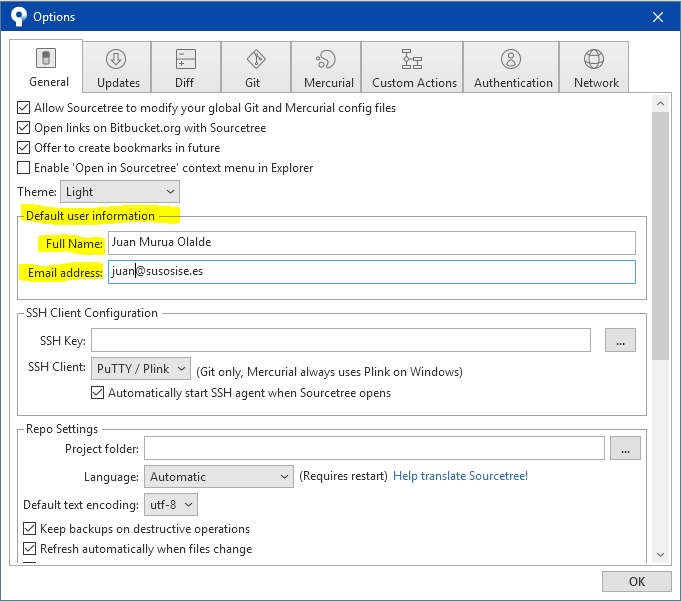
\includegraphics[width=0.65\textwidth]{Sourcetree - configurar datos identificativos generales}

Nota: También es posible indicar unos datos distintos solo para un proyecto concreto, usando el menú `Repository' `Repository Settings...'
\\ 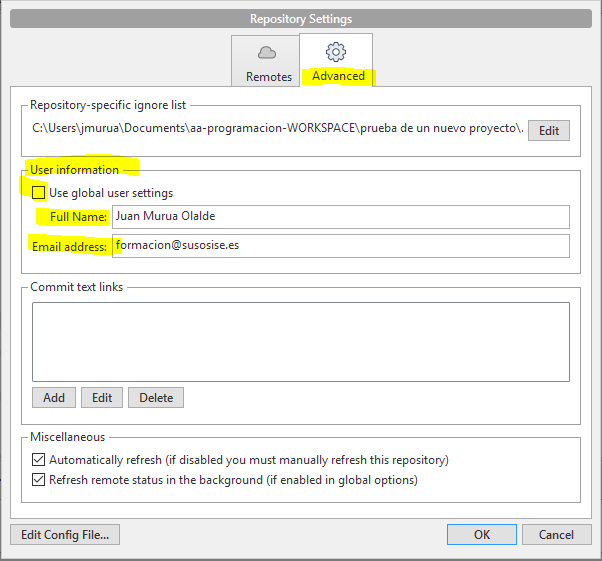
\includegraphics[width=0.65\textwidth]{Sourcetree - configurar datos identificativos para un repositorio}


Para comenzar a trabajar. Crear un nuevo repositorio para un proyecto. Mejor hacerlo en una nueva carpeta.
\\ 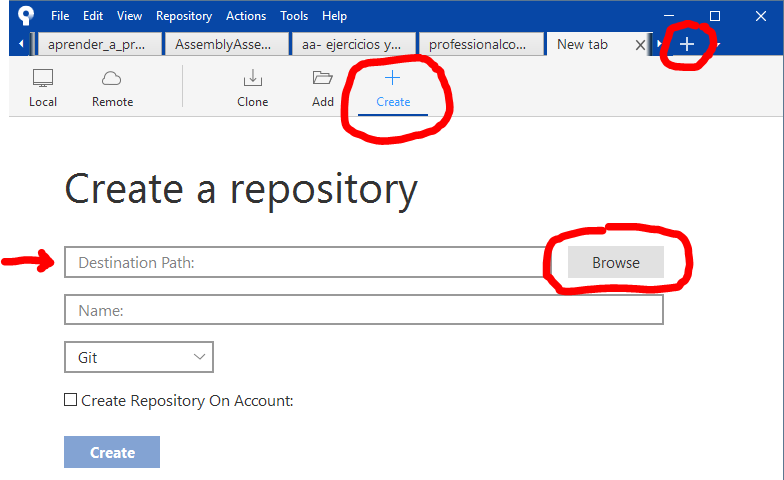
\includegraphics[width=0.8\textwidth]{Sourcetree - dar la orden de crear nuevo repositorio}
\\ 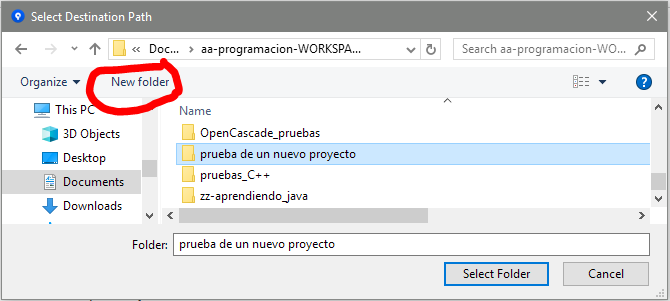
\includegraphics[width=0.8\textwidth]{Sourcetree - crear nueva carpeta en el disco}
\\ 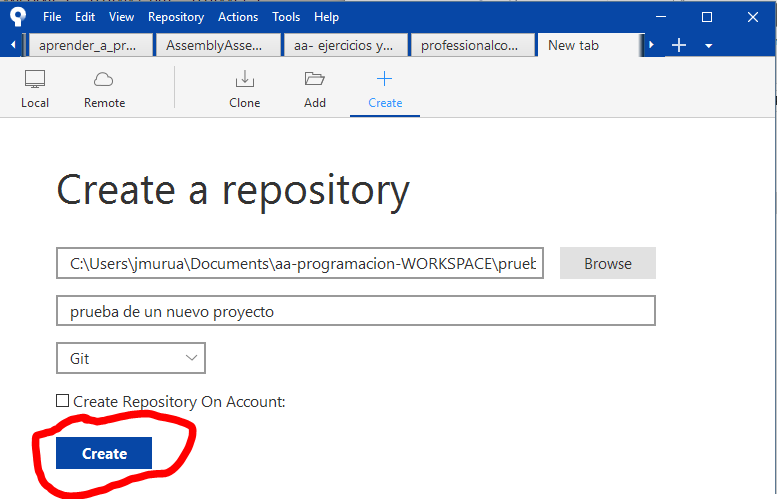
\includegraphics[width=0.8\textwidth]{Sourcetree - crear nuevo repositorio}
\\ 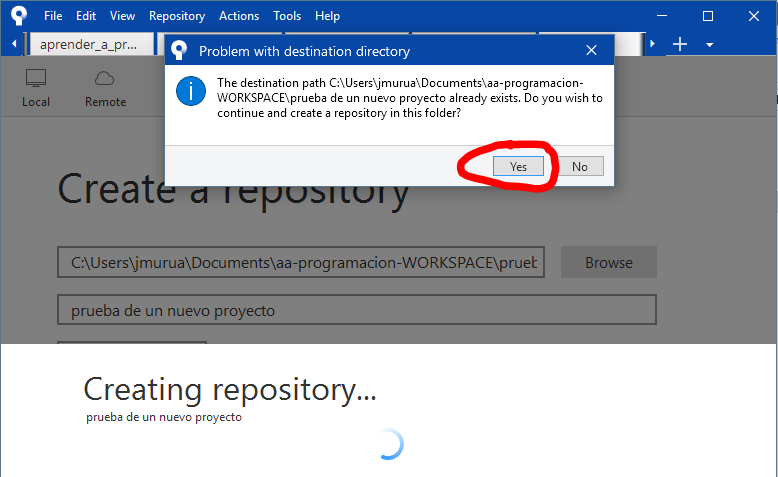
\includegraphics[width=0.8\textwidth]{Sourcetree - aviso al crear nuevo repositorio}

nota: También se puede crear un repositorio desde la línea de comandos, usando la orden `git init' \url{https://git-scm.com/docs/git-init}

Al crear un repositorio, se genera la subcarpeta oculta `.git' bajo la carpeta de proyecto indicada. En esa subcarpeta es donde Git almacenará el contenido y el registro de los cambios que se vayan incorporando en cada ``commit''.
\\ 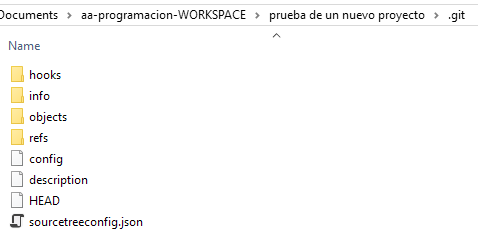
\includegraphics[width=0.7\textwidth]{Sourcetree - contenido de la subcarpeta git}

importante: En la carpeta de proyecto es necesario añadir manualmente un archivo de texto con el nombre `.gitignore'. Este archivo se encarga de que no todo el contenido del proyecto se guarde en el sistema de gestión de versiones. Por ejemplo, los archivos intermedios de compilación, los binarios finales,\ldots no es necesario guardarlos. Ya que son (re)generados automáticamente cada vez que se compila el proyecto..
\\ 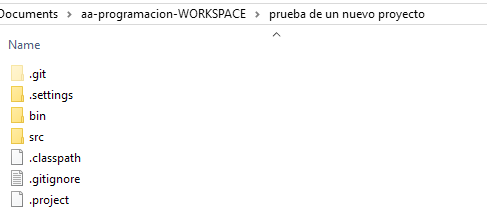
\includegraphics[width=0.7\textwidth]{Sourcetree - contenido de la carpeta con codigo}

Por ejemplo, un trozo del contenido de .gitignore podria ser:
\begin{scriptsize}
\begin{verbatim}
# archivos temporales e instrumentales generados en Java - Eclipse
.metadata/
bin/

# archivos temporales e instrumentales generados en C# - Visual Studio
[Bb]in/
[Dd]ebug/
[Rr]elease/
[Oo]bj/
*.suo
*.user
\end{verbatim}
\end{scriptsize}

Sourcetree (dándole unos segundos para refrescarse tras acceder a su pantalla) nos mostrará en todo momento los archivos que hayan sido modificados desde la última vez que se hizo un ``commit''.
\\ 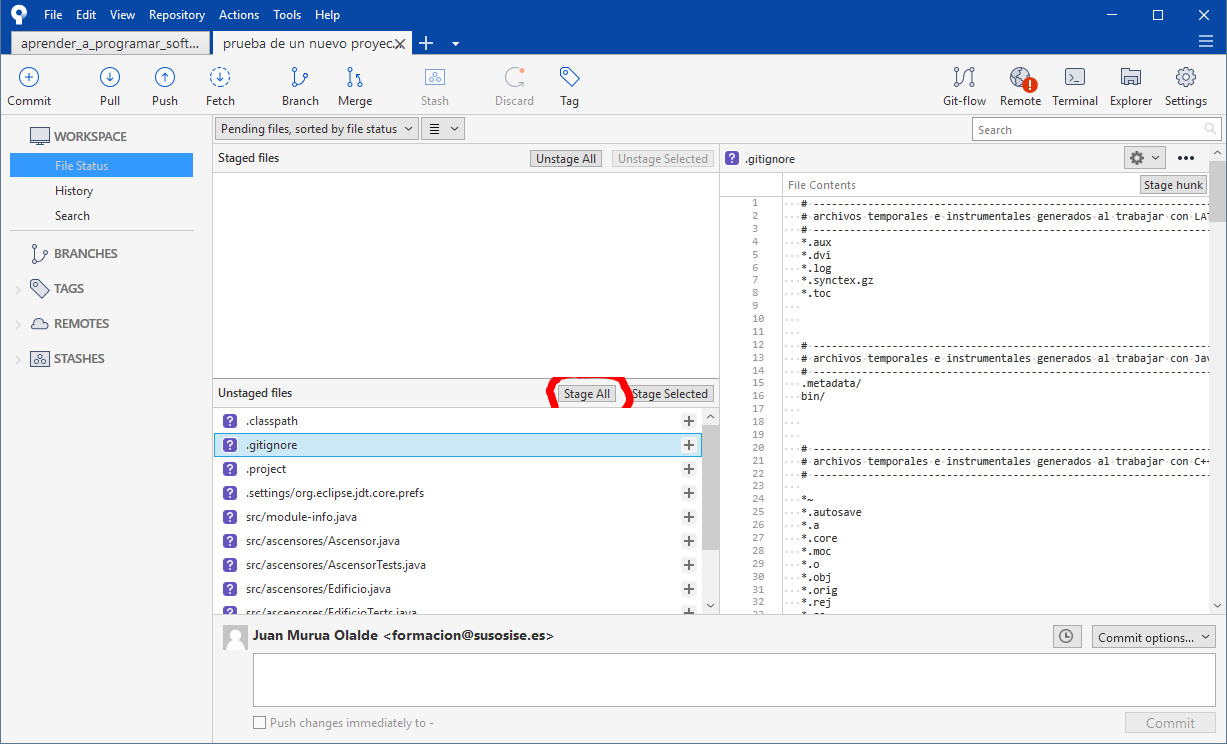
\includegraphics[width=\textwidth]{Sourcetree - stage all}
\begin{small}Nota: Prestar atención al hecho de que la carpeta `bin', que está en la carpeta de código, está siendo ignorada por Sourcetree(Git).\end{small}

Para guardar esos cambios, son necesarios dos pasos:
\begin{enumerate}
\item Poner en el `stage' los archivos de los que se desean guardar cambios clicando el botón que corresponda.
\item Escribir una explicación en el `commit' y clicar en el botón correspodiente.
\end{enumerate}

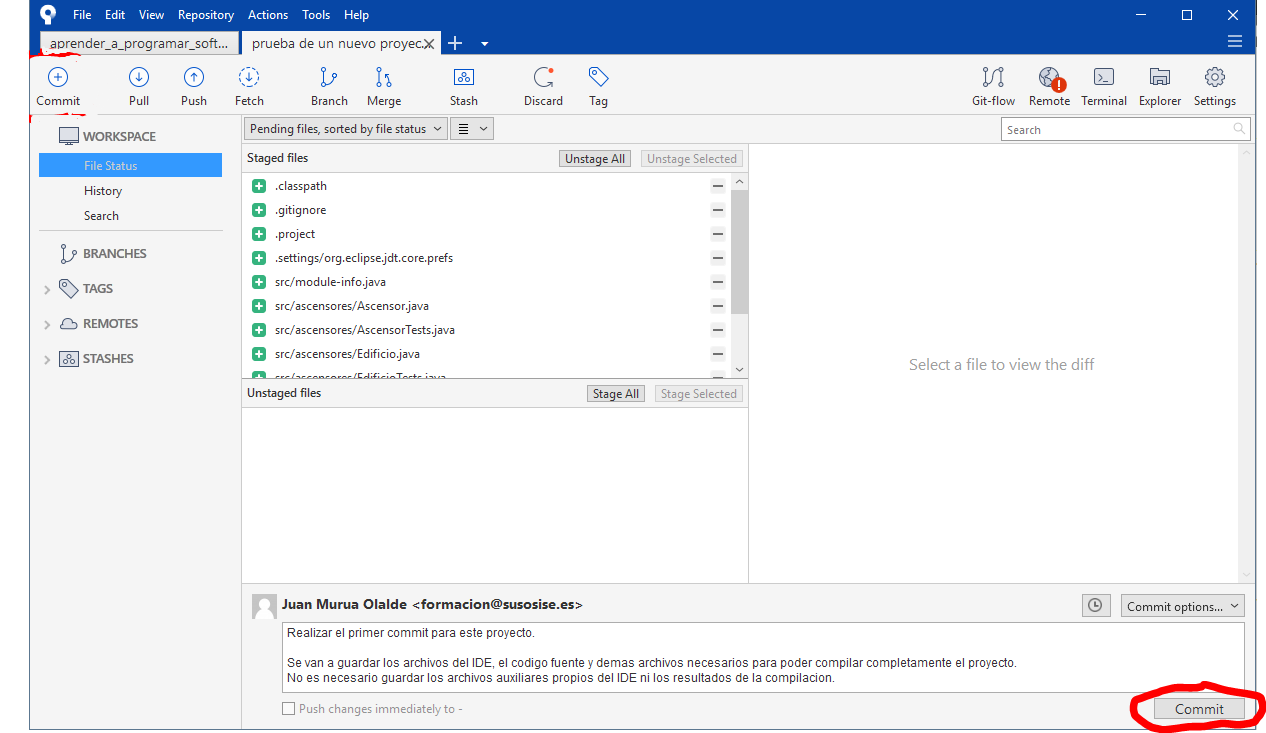
\includegraphics[width=\textwidth]{Sourcetree - commit}
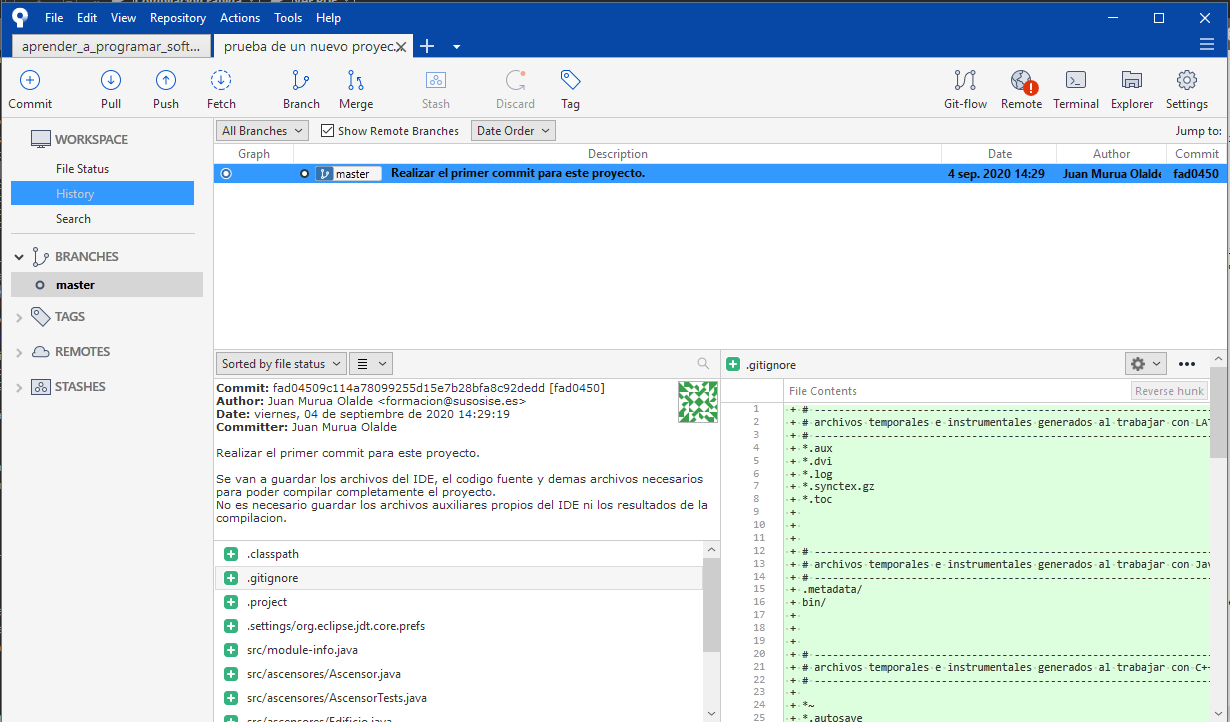
\includegraphics[width=\textwidth]{Sourcetree - rama master tras el primer commit}

La forma básica de trabajar a partir de ahí es la de:
\begin{itemize}
\item Cada vez que se retoma el trabajo en el proyecto, acordarse siempre de comenzar echando un vistazo al estado del proyecto en Sourcetree. Con el tiempo se volverá un hábito saludable.
\item Si se está compartiendo el trabajo con otras personas (es decir, hay repositorios remotos ligados a este repositorio local). Se ha de hacer siempre un \textbf{`pull'} antes de comenzar a trabajar, para traer los cambios que esas otras personas hayan podido realizar. Y comenzar así nuestro trabajo sobre la última versión disponible del proyecto.
\item \textbf{Trabajar\ldots}
\item Cuando se llega a algún punto significativo\ldots, añadir archivos al stage y hacer un \textbf{`commit'} para guardar los cambios hasta ese punto.
\item \textbf{Seguir trabajando\ldots}
\item Cuando se llega a algún punto significativo\ldots, añadir archivos al stage y  hacer un \textbf{`commit'} para guardar los cambios hasta ese punto.
\item \textbf{\ldots}
\item Si se está compartiendo el trabajo con otras personas, acordarse de hacer un \textbf{`push'} para llevar esos commit al repositorio remoto compartido. (Nota: si el trabajo se ha realizado en una rama (`branch') distinta de master, es necesario hacer un `merge' previo al push entre la rama de trabajo y la rama master.) \begin{footnotesize}(Nota: algunos prefieren hacer `rebase's en lugar de `merge's, pero la diferencia entre ambos procesos es un concepto avanzado más allá del alcance de esta breve introducción.)\end{footnotesize} 
\end{itemize}

Un consejo útil: hacer commit con frecuencia, como mínimo uno cada día de trabajo o así. Esto lleva a centrarse en metas concretas que se puedan completar del todo (``done-done'') en un día o así. Potenciando así el saludable hábito de la \textit{programación incremental}: mantener siempre el código en un estado compilable/utilizable y nunca con un montón de frentes abiertos\ldots

Otro consejo útil: compartir (hacer push) con frecuencia. Tener en cuenta que los compañeros no van a ver nuestro trabajo hasta que lo hagamos. Están basando su trabajo sobre el último estado conocido del código. Cuanto más tardemos en compartir, más probabilidades de que se produzcan colisiones entre nuestro trabajo y el suyo por haber escrito dos personas sobre la misma parte del mismo archivo. (\url{https://www.atlassian.com/git/tutorials/using-branches/merge-conflicts})

Un consejo importante: bajo ningún concepto, NUNCA,\ldots intentar corregir un commit ya realizado. Siguiendo el saludable hábito de la \textit{transparencia}, la forma correcta de subsanar un error en un commit es hacer otro commit guardando nuevos cambios correctores y explicando en su comentario la existencia de un error en el anterior commit y que es corregido por este nuevo commit.
\\Git tiene comandos que permiten alterar, revertir o borrar commits ya realizados\ldots ¡pero son un camino seguro al desastre para cualquier persona novata!



\section{Test unitarios}
Los test \textbf{son una parte más del código}. A medida que escribimos código ``para hacer'' algo, escribimos también el correspondiente código ``para comprobar'' que ese algo se hace como se pretendía hacerlo. 

truco: Es más sencillo si trabajamos de forma incremental, en pequeños pasos; cada paso una funcionalidad. Es decir, no esperar a tener una enorme porción de código ``para hacer'' antes de ponernos a escribir sus correspondientes partes de código `para comprobar''.

El orden en que se escriba cada parte no es relevante. Es más, los seguidores del paradigma `Test-driven development' (TDD) recomiendan escribir primero el código ``para comprobar'', ejecutarlo, comprobar que el test falla y escribir luego el código ``para hacer'' que permita al test ejecutarse con éxito.

Los test \textbf{son una red de seguridad} imprescindible para refactorizar y evolucionar(modificar) cualquier programa sin correr demasiados riesgos de romper la funcionalidad existente.

(nota: Todos tendemos a evitar tocar aquello que percibimos como peligroso. Un código sin test tiende, con el tiempo, a convertirse en una serie de ``pastiches'' ligados entre sí sin demasiada coherencia. El miedo lleva a reducir los cambios a los mínimos imprescindibles. Evitando refactorizar lo que ya funciona. E impidiendo así que las nuevas aportaciones se integren con coherencia en el conjunto ya existente.)

Los test \textbf{constituyen una excelente documentación técnica} para el programa. Recogen detalladamente lo que este ha de hacer, todos los requisitos y la intención de diseño. Muchas veces es más sencillo enterarse qué hace un determinado código leyendo sus test que leyendo el propio código. 

(nota: Todos los programadores profesionales sabemos que la otra alternativa: la de documentar el código reflejandolo en algo externo totalmente desligado de él, nunca se mantiene y acaba siempre  desactualizada (es decir, inútil). Sin embargo, los test sí que se mantienen regularmente; de hecho, no hay más que ejecutarlos para ver cuales fallan.)


\subsubsection{Un ejemplo:}
\begin{lstlisting}[frame=single]
public class AnalizadorDeTextos
{
    private String texto;
    private java.util.ArrayList<String> palabras;
    
    public AnalizadorDeTextos(String texto)
    {
        this.texto = texto;
        
        this.palabras = new java.util.ArrayList<String>();
        separarLasPalabras();
    }
    
    private void separarLasPalabras()
    {
        String expresionRegularDeFiltro = "\\s+";
        for (String palabra : texto.split(expresionRegularDeFiltro))
        {
            this.palabras.add(palabra);
        }
    }
    
    public Integer getNumeroDePalabrasEnElTexto()
    {
        return this.palabras.size();
    }
    
    public java.util.ArrayList<String> getListaDePalabrasEnElTexto()
    {
        return this.palabras;
    }

}



import static org.junit.jupiter.api.Assertions.*;
import org.junit.jupiter.api.Assertions;
import org.junit.jupiter.api.Test;

class AnalizadorDeTextosTest
{
    
    @Test
    void testGetNumeroDePalabrasEnElTexto()
    {
   	 AnalizadorDeTextos analizadorSinPuntuacion
                                    = new AnalizadorDeTextos("Esto es una prueba");
   	 assertEquals((Integer)4,      
                     analizadorSinPuntuacion.getNumeroDePalabrasEnElTexto());
   	 
   	 AnalizadorDeTextos analizadorConPuntuacion 
                          = new AnalizadorDeTextos("Esto es una prueba, pardiez.");
   	 assertEquals((Integer)5, 
                     analizadorConPuntuacion.getNumeroDePalabrasEnElTexto());
   	 
   	 AnalizadorDeTextos analizador1 = new AnalizadorDeTextos("prueba");
   	 assertEquals((Integer)1, analizador1.getNumeroDePalabrasEnElTexto());
   	 
   	 AnalizadorDeTextos analizador0 = new AnalizadorDeTextos("");
   	 assertEquals((Integer)0, analizador0.getNumeroDePalabrasEnElTexto());
    }


    @Test
    void testGetListaDePalabrasEnElTexto()
    {
   	 AnalizadorDeTextos analizadorSinPuntuacion 
                                    = new AnalizadorDeTextos("Esto es una prueba");
   	 ArrayList<String> resultadoSinPuntuacion = new ArrayList<String>();
   	 resultadoSinPuntuacion.add("Esto");
   	 resultadoSinPuntuacion.add("es");
   	 resultadoSinPuntuacion.add("una");
   	 resultadoSinPuntuacion.add("prueba");
   	 assertEquals(resultadoSinPuntuacion, 
                     analizadorSinPuntuacion.getListaDePalabrasEnElTexto());
   	 
   	 AnalizadorDeTextos analizadorConPuntuacion 
                          = new AnalizadorDeTextos("Esto es una prueba, pardiez.");
   	 ArrayList<String> resultadoConPuntuacion = new ArrayList<String>();
   	 resultadoConPuntuacion.add("Esto");
   	 resultadoConPuntuacion.add("es");
   	 resultadoConPuntuacion.add("una");
   	 resultadoConPuntuacion.add("prueba");
   	 resultadoConPuntuacion.add("pardiez");
   	 assertEquals(resultadoConPuntuacion, 
                     analizadorConPuntuacion.getListaDePalabrasEnElTexto());
   	 
   	 AnalizadorDeTextos analizador1 = new AnalizadorDeTextos("prueba");
   	 ArrayList<String> resultado1 = new ArrayList<String>();
   	 resultado1.add("prueba");
   	 assertEquals(resultado1, analizador1.getListaDePalabrasEnElTexto());
   	 
   	 AnalizadorDeTextos analizador0 = new AnalizadorDeTextos("");
   	 ArrayList<String> resultado0 = analizador0.getListaDePalabrasEnElTexto();
   	 assertEquals(0, resultado0.size());
    }

}
\end{lstlisting}

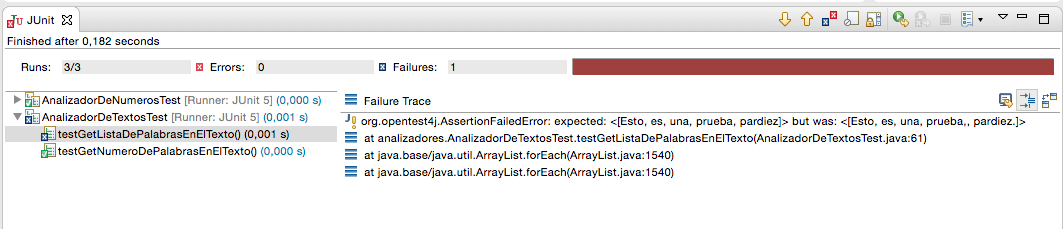
\includegraphics[width=\textwidth]{resultados de JUnit} 

\subsubsection{Otro ejemplo:}
\begin{lstlisting}[frame=single]
public class Ascensor
{
    private int plantaMasBaja;
    private int plantaMasAlta;
    
    private int plantaDondeEstaAhora;
    

    public Ascensor(Integer cantidadDePlantasPorEncimaDeCero, 
                    Integer cantidadDePlantasPorDebajoDeCero)
    {
   	 this.plantaDondeEstaAhora = 0;
   	 if(cantidadDePlantasPorEncimaDeCero > 0 
          && cantidadDePlantasPorDebajoDeCero >= 0)
   	 {
   		 this.plantaMasBaja = cantidadDePlantasPorDebajoDeCero * -1;
   		 this.plantaMasAlta = cantidadDePlantasPorEncimaDeCero;
   	 }
   	 else
   	 {
   		 throw new java.lang.IllegalArgumentException();
   	 }
    }
    
    
    public void IrALaPlanta(Integer planta)
    {
   	 if (planta >= this.plantaMasBaja && planta <= this.plantaMasAlta)
   	 {
   		 this.plantaDondeEstaAhora = planta;
   	 }
    }
    
    public Integer getPlantaDondeEstaAhora()
    {
   	 return this.plantaDondeEstaAhora;
    }
    
    
    public String toString()
    {
   	 return "Este ascensor puede ir desde la planta " 
               + this.plantaMasBaja + " hasta la planta " + this.plantaMasAlta
               + System.lineSeparator()
               + "Ahora esta en la planta " + this.getPlantaDondeEstaAhora();
   	 
    }
    
}


class AscensorTest
{
    @Test
    void Comprobar_situaciones_excepcionales()
    {
   	 assertThrows(java.lang.IllegalArgumentException.class,
   			() -> {Ascensor prueba = new Ascensor(-2, 2);} );
   	 assertThrows(java.lang.IllegalArgumentException.class,
   		      	() -> {Ascensor prueba = new Ascensor(2, -2);} );
   	 
    }
    
    @Test
    void Comprobar_operaciones_normales()
    {
   	 Ascensor ascensorDePruebas = new Ascensor(2,2);
   	 assertEquals((Integer)(0), ascensorDePruebas.getPlantaDondeEstaAhora());
   	 
   	 ascensorDePruebas.IrALaPlanta(1);
   	 assertEquals((Integer)(1), ascensorDePruebas.getPlantaDondeEstaAhora());
   	 
   	 ascensorDePruebas.IrALaPlanta(-1);
   	 assertEquals((Integer)(-1), ascensorDePruebas.getPlantaDondeEstaAhora());
   	 
    }
    
    @Test
    void Comprobar_operaciones_anomalas()
    {   	 
   	 Ascensor ascensorDePruebas = new Ascensor(2,2);
   	 ascensorDePruebas.IrALaPlanta(333);
   	 assertEquals((Integer)(0), ascensorDePruebas.getPlantaDondeEstaAhora());
    }

}
\end{lstlisting}



\subsubsection{Breve introducción a JUnit4}
Aquí se dan cuatro pinceladas para comenzar a trabajar con JUnit4 dentro de Eclipse. Para más detalles, acudir a la web oficial (\url{https://junit.org/junit4/}) o a otras fuentes de información.

En las propiedades del proyecto (menú `Project' `Properties'), en el apartado `Java Build Path', en la pestaña `Libraries', incorporar los dos .jar de biblioteca: hamcrest-core-1.3.jar y junit-4.13.jar

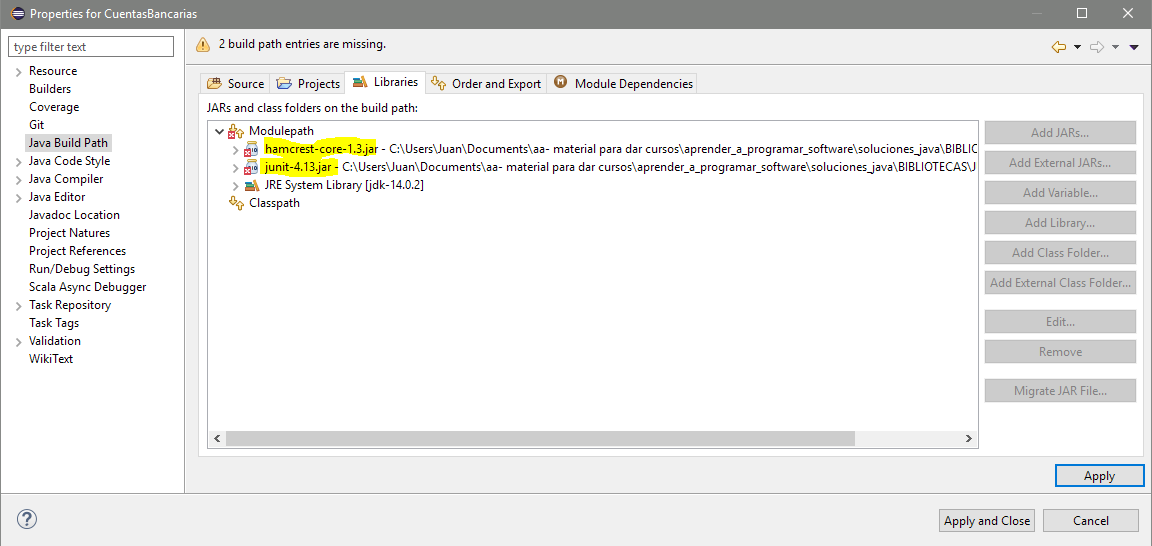
\includegraphics[width=0.9\textwidth]{JUnit4 - poner bibliotecas en Java Build Path del proyecto}

Por cada clase de código, incorporar al proyecto otra clase de test. En las clases de test hay que importar los objetos JUnit que se vayan a utilizar: 
\begin{verbatim}
import org.junit.Test;
import static org.junit.Assert.*;
\end{verbatim}

Dentro de una clase de test, sus métodos(funciones) de test han de ser públicos y se han de identificar con la correspondiente propiedad @Test:
\begin{verbatim}
	@Test
	public void ComprobarAsociacionDeUnaCuentaAlCliente()
	{
		assertEquals(0, clienteDePrueba.getIDsDeLasCuentasAsociadas().size());
		clienteDePrueba.asociarUnaCuentaAlCliente('123456789');
		java.util.ArrayList<String> cuentas = clienteDePrueba.getIDsDeLasCuentasAsociadas();
		assertEquals(1, cuentas.size());
		assertEquals('123456789', cuentas.get(0));
	}
\end{verbatim}
Procurar que el nombre de cada método(función) refleje lo mejor posible la comprobación que realiza. No preocuparse porque los nombres resulten largos.

JUnit tiene soporte directo por parte de Eclipse, así es que los test se ejecutan directamente con clic-dcho `Run As' `JUnit Test'.

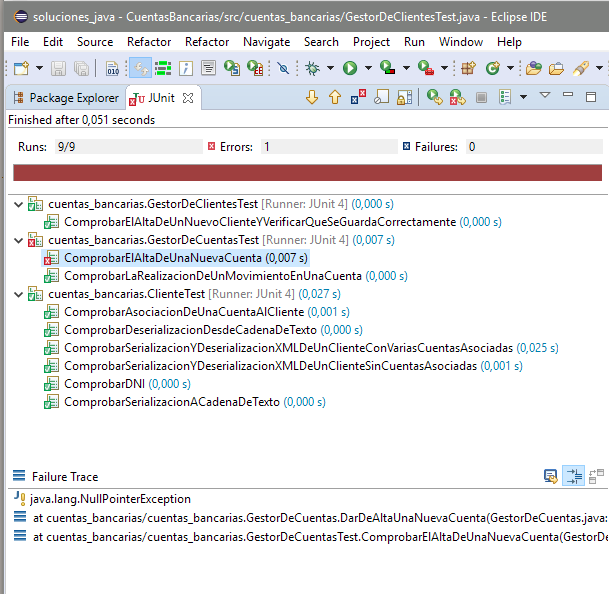
\includegraphics[width=0.8\textwidth]{JUnit4 - ejecucion de los test}



\subsubsection{Breve introducción a QTest}
Aquí se dan cuatro pinceladas para comenzar a trabajar con QTest dentro de Qt Creator. Para más detalles, acudir a la web oficial (\url{https://doc.qt.io/qt-5/qtest-overview.html}) o a otras fuentes de información.


\subsubsection{Breve introducción a los proyectos test de Visual Studio}
Aquí se dan cuatro pinceladas para comenzar a trabajar con test unitarios dentro de Visual Studio. Para más detalles, acudir a la web oficial (\url{https://docs.microsoft.com/es-es/visualstudio/test/getting-started-with-unit-testing?view=vs-2019}) o a otras fuentes de información.


\subsubsection{Breve introducción a unittest}
Aquí se dan cuatro pinceladas para comenzar a trabajar con unittest en Python. Para más detalles, acudir a la web oficial (\url{https://docs.python.org/3/library/unittest.html}) o a otras fuentes de información.




\section{Refactorizar}
Refactorizar: reescribir código sin afectar en nada a lo que este hace.

El código sigue haciendo exactamente lo mismo. Pero se mejora su coherencia interna, se hace más claro de leer, se mejora su mantenibilidad, se evolucionan las técnicas utilizadas, se hace más fácil de modificar, se mejora...

Es importante conocer las ayudas que el editor puede ofrecer a este respecto:
\begin{itemize}
\item Renombrar variables, funciones, clases, módulos,... ; cambiando automáticamente su nombre allá donde han sido utilizadas.
\item Mover variables, métodos, clases,... de una clase, módulo, archivo, carpeta,... a otra ; actualizando automáticamente las referencias allá donde han sido utilizadas (o marcando dichos puntos, si necesitan ajuste manual).
\item Cambiar parámetros en la signatura de una función o método ; actualizando automáticamente los puntos donde ha sido utilizada (o marcando dichos puntos, si necesitan ajuste manual).
\item Extraer un tozo de código a su propia función; definiendo automáticamente los parámetros de entrada y de salida necesarios.
\item etc.
\end{itemize}

Y nunca está de más destacar la red de seguridad aportada por los test unitarios. Tras cada refactorización, los test nos aseguran que el código sigue haciendo lo mismo que hacia antes, (o nos avisan de los puntos donde hemos alterado alguna funcionalidad sin querer).\footnote{Ver más información sobre estas y otras herramientas de programación en el capítulo 1 ``Herramientas'' del documento \url{https://www.susosise.es/documentos/Proyecto_Software.pdf}}




\chapter{Interfaz gráfico de usuario: GUI \small{(Graphic User Interface)}}


\section{Formas de construirlos}
Hay dos formas de definir las pantallas:

\subsection{Indicando ubicaciones y dimensiones fijas}
Dibujando tal cual el interfaz a presentar. Es decir, dando prescripciones exactas de donde ha de ir cada elemento.

Tiene la ventaja de ser sencillo y evidente, ya que es totalmente estático.

Pero tiene la pega de que:
\begin{itemize}
\item Puede resultar imposible acceder a ciertos controles, si se trabaja en una pantalla de menos resolución que la inicialmente prevista.
\item Puede visualizarse con tamaño diminuto, si se trabaja en una pantalla de mucha más resolución y densidad de la inicialmente prevista.
\end{itemize}

\subsection{Indicando relaciones y recomendando dimensiones}
Dando intenciones de diseño y dejando que sea el propio sistema quien dibuje el interfaz, según pueda hacerlo en cada ocasión. Para ello:
\begin{itemize}
\item Se elige una distribución general de la pantalla (layout). Esta distribución dictará las diferentes zonas y las formas generales de acomodar elementos.
\item Se ponen componentes dentro de cada zona, en un determinado orden de colocación e indicando los márgenes a respetar para dimensiones y espaciados (mínimas, preferidas, máximas).
\end{itemize}

Tiene la ventaja de adaptarse automáticamente a diversos tamaños y formatos de pantalla. Algo muy útil hoy en día, ya que la aplicación será utilizada desde diversos dispositivos: sobremesas, portátiles, tabletas, móviles,... con pantallas de diferentes resoluciones y densidades.

Pero tiene la pega de ser más complejo de definir y de requerir ensayos prueba/error para comprobar su correcto comportamiento en diversos escenarios de uso. (Además, al ser dinámico, puede no resultar siempre exactamente como queremos que quede.)

\section{Event Loop , Event Dispatcher ::: Reaccionar a lo que sucede \\ en la pantalla, en el ratón o en el teclado}
(nota: Para una descripción general de cómo funciona este sistema, ver más adelante la sección \ref{eventos} \nameref{eventos}.)

\section{Responsive GUI ::: Reaccionar a lo que sucede \\ en el interior de la aplicación}
`WorkerThread' y otros sistemas para ejecutar el código en diversas hebras de ejecución coordinadas entre sí. (Sin perder de vista que, normalmente, la hebra principal suele ser aquella donde corre el interfaz gráfico --donde ha arrancado la aplicación y desde la que se inician las demás hebras--.)

\section{Elementos habituales en los GUIs}

Un poco de historia y curiosidades:
\begin{itemize}
\item Los primeros prototipos: Engelbart y ``la madre de todas las demos''. \url{https://www.youtube.com/playlist?list=PLCGFadV4FqU2yAqCzKaxnKKXgnJBUrKTE}
\item El primer equipo viable en los EEUU: Xerox Alto.
\\ \url{https://es.wikipedia.org/wiki/Xerox_Alto}
\item El primer equipo viable en Europa: Oberon 
\\ \url{https://en.wikipedia.org/wiki/Oberon_(operating_system)}
\\ \url{http://www.projectoberon.com/}
\item El primer sistema comercial con éxito: Apple Macintosh
\\ \url{https://es.wikipedia.org/wiki/Macintosh}
\end{itemize}

\subsection{Controles con los que el usuario puede interactuar}

Los más habituales suelen ser:
\begin{itemize}
\item tipo ``Label'': algo donde mostrar texto.
\item tipo ``TextBox'': algo donde introducir texto.
\item tipo ``Button'' o ``PushButton'': algo donde hacer clic para desencadenar una acción.
\item tipo ``RadioButton'': algo para elegir una, y solo una, de entre varias opciones.
\item tipo ``CheckBox'': algo para activar/desactivar una opción.
\item tipo ``Slider'': algo para indicar cantidades de forma continua, deslizándose entre un mínimo y un máximo.
\item tipo ``ListView'' o ComboBox'': algo para elegir uno, o varios, de entre una lista (corta) de elementos predefinidos.
\item tipo ``TreeView'': algo para elegir uno, o varios, de entre una colección (larga) de elementos predefinidos organizados de forma arbórea.
\item tipo ``ProgressBar'': algo con lo que mostrar el progreso de una tarea larga.
\item tipo ``PictureBox'': algo donde mostrar imágenes.
\item tipo ``Player'': algo donde mostrar vídeos.
\item tipo ``Table'': algo donde interactuar con datos tabulares.
\item tipo ``Scroll'': algo para permitir desplazar el contenido y así poder visualizarlo cuando no cabe entero en el espacio previsto para él.
\end{itemize}

\subsection{Distribuciones generales con las que organizar la pantalla}

Las más habituales suelen ser:
\begin{itemize}
\item tipo ``panel'': se usan para agrupar varios componentes y poder así colocarlos como si fueran un solo componente.
\item tipo ``flow'': los componentes se colocan de forma secuencial uno detrás de otro, en sentido horizontal o en sentido vertical.
\item tipo ``grid'': los componentes se colocan en las casillas de una rejilla con un cierto número de columnas y de filas. 
\item tipo ``boxes'': el espacio se distribuye en zonas fijas donde se colocan componentes; normalmente esas zonas suelen ser cinco: arriba (norte), a la izquierda (oeste), en el centro, a la derecha (este), abajo (sur).
\item tipo ``cards'': se dispone de varias páginas, permitiendo saltar fácilmente de una a otra (usualmente mediante unas pestañas o algo similar).
\end{itemize}
Estas distribuciones (`layouts') se pueden combinar entre sí. Por ejemplo: podemos poner un ``flow'' dentro de una celda concreta de un ``grid'', podemos poner un determinado ``grid'' dentro de la zona centro de un ``boxes'', podemos poner diferentes ``grid''s en las diferentes páginas de un ``cards'', etc.

\subsubsection*{Algunos enlaces prácticos \begin{footnotesize}(Una imagen vale más que mil palabras\ldots)\end{footnotesize}}

A Visual Guide to Java Swing Layout Managers: \url{https://docs.oracle.com/javase/tutorial/uiswing/layout/visual.html}
\\JavaFX Layout Panes: \url{https://docs.oracle.com/javafx/2/layout/builtin_layouts.htm}

QT Layout Management: \url{https://doc.qt.io/qt-5/layout.html}

.NET WPF Layouts, a Visual Quick Start: \url{https://www.codeproject.com/Articles/30904/WPF-Layouts-A-Visual-Quick-Start}
\\WPF Layout System: \url{https://docs.microsoft.com/es-es/dotnet/desktop/wpf/advanced/layout?view=netframeworkdesktop-4.8}

Python Tkinter Grid Geometry Manager: \url{https://tkdocs.com/tutorial/grid.html}


\section{Ejercicios}\label{ejercicios_gui}


\subsection{Hello, Benzirpi.}\label{ejercicio_hellobenzirpi}
Algo sencillo para empezar: un texbox donde teclear un nombre y un botón que rellena otro textbox (de solo lectura) con un saludo a ese nombre.
\\ 
\includegraphics[width=\textwidth]{HelloBenzirpi - pantallazo - Java}

\subsection{Bocatas}\label{ejercicio_bocatas}
Algo sencillo para elegir opciones: unos cuantos radiobuttons y checkboxes.
\\ 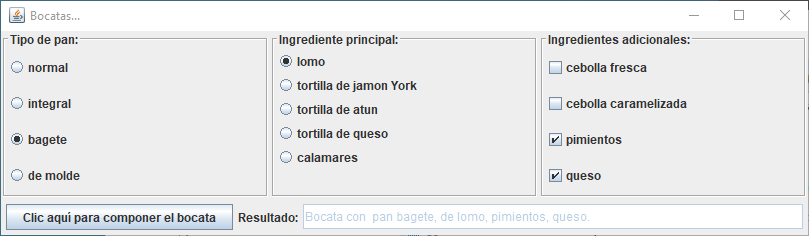
\includegraphics[width=\textwidth]{Bocatas - pantallazo - Java}

\subsection{Selección plana}\label{ejercicio_selecionplana}
Algo sencillo para elegir un elemento de una lista desplegable o de una lista abierta.
\\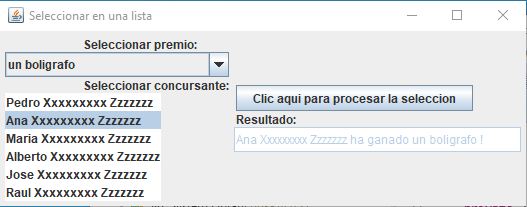
\includegraphics[width=\textwidth]{Seleccion Plana - pantallazo - Java}

\subsection{Diálogos estándares}\label{ejercicio_dialogos}
Manejo de los diálogos del sistema operativo para: seleccionar carpetas, seleccionar archivos, seleccionar colores,...
\\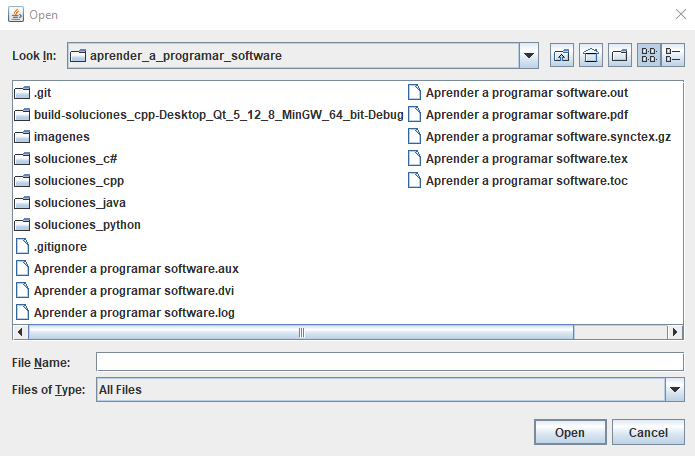
\includegraphics[width=\textwidth]{Dialogos Estandares - JFileChooser - Java}
\\\\
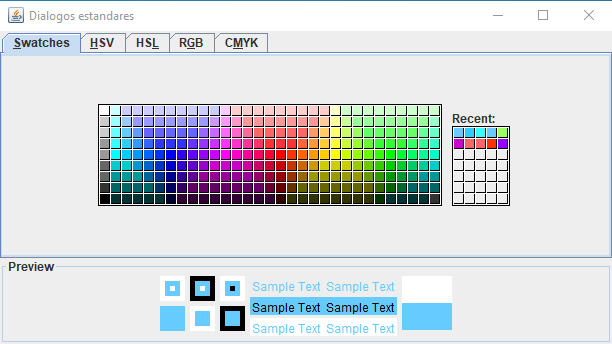
\includegraphics[width=0.5\textwidth]{Dialogos Estandares - JColorChooser - Swatches - Java}
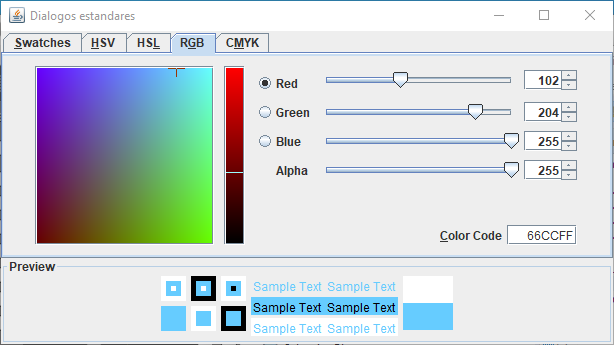
\includegraphics[width=0.5\textwidth]{Dialogos Estandares - JColorChooser - RGB - Java}

\subsection{Scroll}\label{ejercicio_scroll}
Cuando se ha de mostrar un contenido que no cabe en el espacio disponible, se puede recurrir a unos deslizadores (scrollbars) horizontales o verticales para permitir desplazar dicho contenido dentro del espacio disponible.
\\ 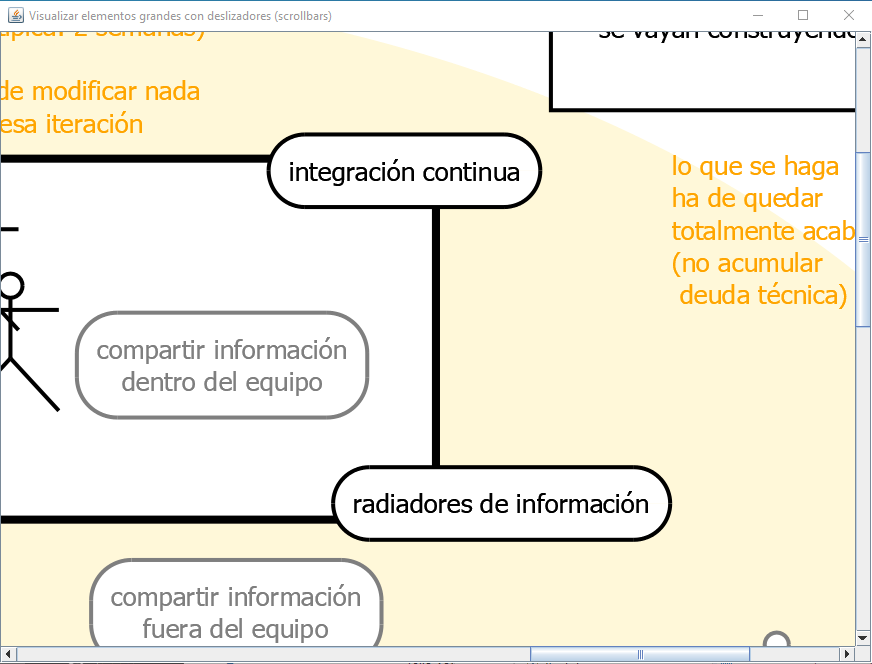
\includegraphics[width=0.8\textwidth]{Scroll - pantallazo - Java}

\subsection{Split}\label{ejercicio_split}
Cuando se desea permitir al usuario modificar sobre la marcha el espacio dedicado dentro de la ventana a los componentes dentro de ella, se puede recurrir a un separador ajustable entre zonas (spliter).
\\ 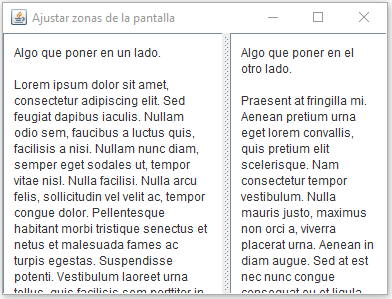
\includegraphics[width=0.8\textwidth]{Split - pantallazo - Java}

\subsection{Calendario}\label{ejercicio_calendario}
Pedir una fecha mostrando un calendario.

\subsection{Selección arbórea}\label{ejercicio_selecionarborea}
Presentar elementos con estructura jerárquica en árbol, navegar a través de ella mostrando u ocultando ramas, seleccionar algún elemento, y hacer algo con él (por ejemplo, mostrar información detallada de ese elemento concreto).

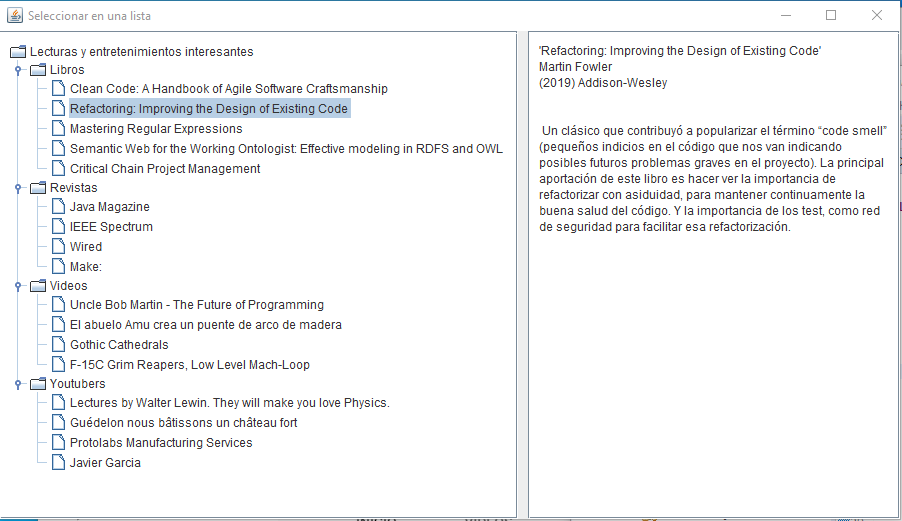
\includegraphics[width=\textwidth]{Seleccion Arborea - pantallazo - Java}


\subsection{Barra de progreso}\label{ejercicio_barradeprogreso}
Cuando se desencadena una tarea larga, es conveniente mantener al usuario informado de cómo va progresando dicha tarea. Así se evita dar la impresión que el sistema se ha colgado.

nota: No suele ser sencillo. Se ha de recurrir a la multitarea para conseguir que el interfaz de usuario (main thread) se vaya refrescando periódicamente mientras se está ejecutando la tarea (worker thread). Pero es algo tan necesario que casi todos los entornos de programación cuentan con algún mecanismo específico para implementar esa comunicación periódica.

Una sugerencia de ejercicio para practicar:
\\ 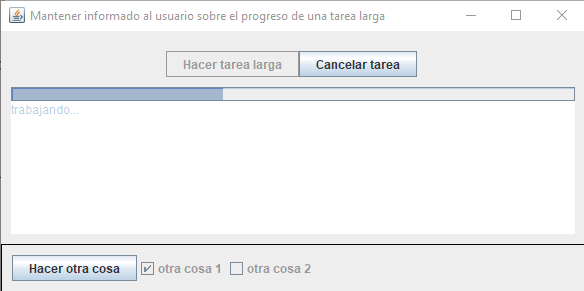
\includegraphics[width=0.7\textwidth]{BarraDeProgreso - pantallazo - Java}

Una lectura interesante: \url{https://www.oracle.com/technical-resources/articles/javase/swingworker.html}


\subsection{Internacionalización (i18n) y localización (L10n)}\label{ejercicio_localizacion}
\begin{itemize}
\item Internacionalización (i18n) son los mecanismos para adaptar el software a distintos idiomas y países.
\item Localización (L10n) son los mecanismos para adaptar el software a los distintos usos y costumbres de cada país: moneda, pesos y medidas, formatos numéricos, unidades de medida, formatos de fecha/hora, convenciones culturales, sentido de escritura,\ldots
\end{itemize}

Ambos dos son aspectos muy importantes para cualquier software que no sea algo pequeño ``de andar por casa''. Y, aún en estos, hay que tener en cuenta que muchas veces crecen y acaban desplegándose por multitud de sitios a donde no se había previsto que llegaran.

Tanto la internacionalización como la localización son prácticamente imposibles de implementar ``a posteriori''. Es decir, se han de ir incorporando desde el primer momento; desde la primera línea de código que se escriba.

Si conocemos y nos sentimos cómodos usando los mecanismos que tenga nuestra plataforma de desarrollo para facilitar esos aspectos. No nos costará mucho más utilizarlos en todos nuestros trabajos; aunque en ese momento estemos pensando en un solo idioma y un solo país. Así, si mas tarde se han de incorporar más idiomas o más países, el camino estará preparado.


\subsection{Ayudas y documentación}\label{ejercicio_ayudas}
Es importante conocer los mecanismos que tenga nuestra plataforma de desarrollo para mostrar documentación de forma dinámica: indicaciones al poner el ratón un tiempo quieto sobre un determinado elemento(tooltips), acceso al manual de uso (ayuda, tecla F1), advertencias directas para algunos aspectos especialmente delicados (pop-ups), etc.

Son aspectos importantes si se van a desarrollar programas de una cierta envergadura. Programas que vayan a ser usados por muchas personas distintas, a lo largo de mucho tiempo.

\subsubsection*{Algunas recomendaciones}
Creo que es mejor no incordiar mucho a los usuarios en su día a día. Suele ser suficiente con disponer de:
\begin{itemize}
\item Unos tooltips cortos y precisos acerca de lo que hace cada parte del interface. Tooltips que solo aparezcan si el usuario deja manifiestamente el ratón quieto durante unos 2 segundos sobre algo. 
\item Y un menú o botón de `Ayuda' bien visible, que abra el manual de usuario.
\end{itemize}

Por experiencia sé que casi nadie se lee el manual de usuario. Ni aún en el caso de que esté bien redactado, sea claro y sea ameno.

Pero aún así, creo que merece la pena dotar a nuestros programas de una buena documentación. Algo que realmente permita permita a una persona curiosa aprender la filosofia de funcionamiento del programa y los conceptos principales involucrados en su manejo.

Escribir una mera recopilación de cómo hacer qué, menú a menú y botón a botón, solo por cumplir el expediente, no merece la pena. Además de ser inútiles, han sido ese tipo de manuales los que han dado tan mala fama a los manuales de usuario.

De ponerse a producirlo, suele ser más rentable enfocar el manual de usuario como un curso de autoestudio.
\\Si además se le dota de un buen índice de temas, podrá ser utilizado también, en cierta medida, como referencia puntual para resolver dudas.






\chapter{Objetos: clases e instancias}

\section{Encapsulación}
En la programación orientada a objeto, cada módulo (clase)(objeto) contiene todo lo que necesita para realizar una tarea o misión concreta: 
\begin{itemize}
\item tanto los datos (propiedades),
\item como el comportamiento (métodos).
\end{itemize}

Y se garantiza que ningún objeto pueda interferir en los entresijos internos de otro. Un objeto solo puede interactuar con otro a través de los caminos expresamente habilitados para ello (propiedades o métodos declarados como ‘public’).

nota: ver más detalles más adelante, en la sección \ref{oop} \nameref{oop}.

\section{Polimorfismo}
Es la posibilidad de definir varias funciones (métodos) con el mismo nombre, pero con diferentes signaturas (diferencias en alguno de los parámetros de entrada o en los datos de salida).

\section{Herencia}
Se utiliza cuando hay varias clases similares, clases que comparten todas ellas algunas propiedades y métodos comunes que son idénticos en todas ellas. 

Es posible definir una clase madre con la parte común, y luego derivar varias clases hijas a partir de ella. Todas las clases hijas tienen automáticamente todo lo que tiene la clase madre, más lo que se añada de forma particular para cada una de ellas.

Cuando se vaya a utilizar solo su parte común, podemos declarar variables, parámetros o colecciones del tipo madre, para referirnos o contener instancias de cualquiera de las clases hijas.

\section{Sobrecarga de funciones (overwrite)}
Se utiliza junto con la herencia. Cuando alguna clase hija necesita hacer algo diferente en la implementación interna de alguno de los métodos comunes que recibe de la clase madre. Puede redefinir ese método sobreescribiendolo (overwrite) con una declaración propia. 

\section{Interface (clase abstracta)}
Se utiliza cuando se necesitan unos ciertos métodos con una misma signatura concreta (parámetros de entrada y salida concretos) en varias clases distintas. 

Según cada clase, esos métodos comunes pueden realizar trabajos internos distintos. Pero para un tercero que vaya a usar objetos de alguna de esas clases, todos ellos se manejan igual.

(nota: Se podría utilizar herencia, pero habría que sobreescribir los métodos en todas las clases hijas. La clase madre tan solo dictará la signatura de los métodos. Y eso es precisamente lo que hace un interface.)

Cuando una clase dice que implementa un interface, el compilador le obliga a que implemente todos y cada uno de los métodos de ese interface. Los puede implementar como quiera, pero ha de implementarlos todos; y ha de implementarlos respetando escrupulosamente las signaturas (los parámetros de entrada y salida) definidas.

Cuando se vaya a utilizar solo su parte común, podemos declarar variables, parámetros o colecciones del tipo del interface. Para referirnos o contener instancias de objetos de cualquiera de las clases que implementen dicho interface.

\section{Cuándo usar herencia y cuándo interface}
Ambas se utilizan cuando se ha de garantizar que un cierto número de clases/objetos tienen ciertos elementos comunes a todos ellos; Permitiendo así ser utilizados en ciertas ocasiones como si todos fueran el mismo tipo de objeto. Pero, ¿cuándo usar herencia y cuando interfaz?

Algunas reglas prácticas:
\begin{itemize}
\item Cuando la parte de código común a todas las clases/objetos es mucho mayor que la parte específica de cada cual $\Rightarrow$ implementar la parte común en una clase madre de la cual se derivarán las clases hijas específicas.
\item Cuando la parte de código común a todas las clases/objetos se preve que va a ser muy estable en toda la vida del software $\Rightarrow$ implementar la parte común en una clase madre de la cual se derivarán las clases hijas específicas.
\item Cuando la parte de común a todas las clases/objetos es mucho menor que la parte específica de cada cual $\Rightarrow$ definir la parte común en un interface y obligar a las clases a implementar dicho interface.
\end{itemize}
En caso de duda $\Rightarrow$ Interface suele ser la opción más clara y flexible cara a futuras modificaciones o ampliaciones.

Un aviso: Si la herencia a un nivel (madre$\rightarrow$hijas) suele ser complicada a veces. La herencia a más niveles (madre$\rightarrow$hijas$ \rightarrow$nietas\ldots), suele ser camino con muchas probabilidades de problemas en un futuro. Cuando se vea necesaria multiherencia en alguna aplicación, mejor repensar de nuevo la arquitectura para ver si realmente es o no imprescindible.

\section{Factorias para ``fabricar'' objetos (inyección de dependencias)}
Se utiliza cuando una clase A necesita utilizar objetos de otra clase X, pero no puede o no conviene que los instancie por sí misma. Se suele resolver definiendo una clase factoría capaz de instanciar objetos de diversas clases según los parámetros que se le pasen. La clase A utiliza esa factoría para obtener el objeto que necesita en cada momento.

Un caso de uso bastante típico es cuando el tipo concreto de objeto X a utilizar no se conoce hasta el momento en que el programa está funcionando (tiempo de ejecución); pudiendo ser de un tipo en una ocasión y de otro tipo en otra. Haciendo así imposible preverlo directamente en el código (tiempo de compilación).

Otro caso de uso bastante típico es cuando un objeto X es costoso de crear (por ejemplo, implica una conexión auditada y encriptada con una base de datos remota) y se necesita para los test unitarios de una determinada clase A. Utilizando A desde un test, se puede indicar a la factoria que le suministre un objeto similar a X (con la misma forma funcional externa) pero más sencillo de instanciar y reducido a la mínima expresión necesaria para el test (pseudo-objeto, ``mock'').

\begin{footnotesize}
Un ejemplo ilustrativo:

La clase A utiliza un controlador de datos X para adquirir una lista de clientes llamando a su método getClientesDeLaProvincia(provincia). Pero unas veces los datos están en una base de datos remota y otras veces en un archivo XML local, (es decir, unas veces usa el controlador `GestorDeDatosSQL' y otras usa el controlador `GestorDeDatosXML', ambos dos controladoresX implementando un interfaceX que incluye el método `getClientesDeLaProvincia(provincia)'.
\\Se podria resolver con algo así como este código:
\begin{verbatim}
...
String tipoDeFuenteDeDatos;
InterfaceX fuenteDeDatos;
ArrayList<Cliente> clientes;
...
if (tipoDeFuenteDeDatos == 'SQL')
{
  fuenteDeDatos = new GestorDeDatosSQL();
{
else if (tipoDeFuenteDeDatos == 'XML')
{
  fuenteDeDatos = new GestorDeDatosXML();
}
...
clientes = fuenteDeDatos.getClientesDeLaProvincia('Cordoba');
...
\end{verbatim}
Pero ¿qué pasa si luego queremos extender a otros controladores, como por ejemplo a `GestorDeDatosJSON' o `GestorDeDatosSemanticos'?...\\
Podemos ampliar la construcción if-elseif en el código en la clase A; \textit{pero el trabajo de esa clase es procesar datos de clientes, no el saber de donde proceden esos datos}. Quedaria más limpio si liberamos a la clase A de esa responsabilidad extra, adjudicando esa tarea a una clase específica ad-hoc (una factoria) encargada de crear los gestores de datos necesarios. De este modo, la clase A se veria simplificada:
\begin{verbatim}
...
String tipoDeFuenteDeDatos;
InterfaceX fuenteDeDatos;
ArrayList<Cliente> clientes;
...
fuenteDeDatos = FactoriaDeGestores.getGestorDeDatos(tipoDeFuenteDeDatos);
...
clientes = fuenteDeDatos.getClientesDeLaProvincia('Cordoba');
...
\end{verbatim}
Y toda la parte de:
\begin{verbatim}
...
if (tipoDeFuenteDeDatos == 'SQL')
{
  return new GestorDeDatosSQL();
{
else if (tipoDeFuenteDeDatos == 'XML')
{
  return new GestorDeDatosXML();
}
else if (tipoDeFuenteDeDatos == 'JSON')
{
  return new GestorDeDatosJSON();
}
else if (tipoDeFuenteDeDatos == 'RDF')
{
  return new GestorDeDatosSemanticos();
}
...
\end{verbatim}
iria dentro del método `getGestorDeDatos(tipo)' de la clase `FactoriaDeGestores'.

\end{footnotesize}



\section{Ejercicios y ejemplos}

\url{https://github.com/JuanMuruaOlalde/sugerencias-para-practicar-programacion/tree/main/CuentaBancaria}

\url{https://github.com/JuanMuruaOlalde/sugerencias-para-practicar-programacion/tree/main/Areas_y_Perimetros}

\url{https://github.com/JuanMuruaOlalde/sugerencias-para-practicar-programacion/tree/main/Ascensores}

\url{https://github.com/JuanMuruaOlalde/sugerencias-para-practicar-programacion/tree/main/CuentasBancarias}

\url{https://github.com/JuanMuruaOlalde/sugerencias-para-practicar-programacion/tree/main/Excursiones}

\url{https://github.com/JuanMuruaOlalde/Albaranes}

\url{https://github.com/JuanMuruaOlalde/Hotel}






\chapter{Datos en memoria de trabajo}


\section{Estructuras lineales (arrays, colas,\ldots)}
Han sido modo básico de almacenar información desde los primeros tiempos de la informática. Consisten en una serie lineal contigua de datos, uno detrás de otro; con soporte para las operaciones de añadir, leer, modificar y eliminar elementos de la secuencia.

La estructura lineal más básica es el típico array. Por ejemplo, en C
\begin{lstlisting}[frame=single]
void Usar_un_array_c()
{
    char colores[5][12];
    strcpy(colores[0], "rojo");
    strcpy(colores[1], "azul");
    strcpy(colores[2], "verde");
    strcpy(colores[3], "naranja");
    strcpy(colores[4], "amarillo");

    strcpy(colores[2], "gris");

    for(int i = 0; i < 5 ; i++)
    {
   	 printf("%s\n", colores[i]);
    }

}
\end{lstlisting}
Por ejemplo, en C++
\begin{lstlisting}[frame=single]
void Usar_un_array()
{
    std::array<std::string, 5> colores = {"rojo", "azul", "verde", 
                                          "naranja", "amarillo"};
    colores[2] = "gris";

    for(const auto& color : colores)
    {
   	 std::cout << color << std::endl;
    }

}
\end{lstlisting}
Por ejemplo, en java
\begin{lstlisting}[frame=single]
    public static void OrdenacionBoubleSort()
    {
   	 int CANTIDADDEELEMENTOS = 5;
   	 Double[] ristraDeNumeros = new Double[CANTIDADDEELEMENTOS];
   	 ristraDeNumeros[0] = 4.6;
   	 ristraDeNumeros[1] = 2.1;
   	 ristraDeNumeros[2] = 7.8;
   	 ristraDeNumeros[3] = 5.0;
   	 ristraDeNumeros[4] = 6.2;
   	 System.out.println("ristra original:");
   	 for(int i = 0 ; i < CANTIDADDEELEMENTOS; i++)
   	 {
   	     System.out.println(ristraDeNumeros[i]);
   	 }

   	 for(int i = 0 ; i < CANTIDADDEELEMENTOS - 1 ; i++)
    	 {
            for(int j = 0 ; j < CANTIDADDEELEMENTOS - i - 1 ; j++)
            {
                if(ristraDeNumeros[j] > ristraDeNumeros[j+1])
            	   {
                	Double temporal = ristraDeNumeros[j];
                	ristraDeNumeros[j] = ristraDeNumeros[j+1];
                	ristraDeNumeros[j+1] = temporal;
            	   }
            }
    	 }
   	 
   	 System.out.println("ristra después de ordenarla:");
   	 for(int i = 0 ; i < CANTIDADDEELEMENTOS; i++)
   	 {
   		 System.out.println(ristraDeNumeros[i]);
   	 }
   	 
    }
\end{lstlisting}

Según el tipo de tarea para la que esté optimizada, entre las estructuras de capacidad fija se pueden distinguir:
\begin{itemize}
\item ARRAYs: Están pensados para recorrerse secuencialmente, de principio a fin. Son eficientes para insertar/eliminar registros en el final de la serie o para leer/modificar un registro cualquiera sabiendo la posición (índice) que ocupa dentro de la serie. Otras operaciones son más costosas, por ejemplo: insertar un registro en una posición concreta implica ``empujar'' los posteriores para hacer sitio al recien llegado; eliminar un registro concreto implica  ``mover'' los posteriores para cubrir el hueco; buscar por contenidos implica ir leyendo toda la serie hasta dar con el registro deseado;...
\item COLAs (array FIFO) (QUEUE): Están pensadas para que sea eficiente añadir nuevos registros y recuperarlos en sentido directo (primero en entrar, primero en salir). Suelen tener solo dos operaciones: meter (enqueue) y sacar (dequeue).
\item PILAs (array LIFO) (STACK): Están pensadas para que sea eficiente añadir nuevos registros y recuperarlos en el sentido inverso (último en entrar, primero en salir). Suelen tener solo dos operaciones: poner (push) y quitar (pop).
\end{itemize}

Y entre las estructuras de capacidad variable se pueden distinguir:
\begin{itemize}
\item LISTAS ENCADENADAS: Están pensadas para que sea eficiente recorrerlas desde el principio hacia el final y para insertar/eliminar registros en cualquier punto de la lista.
\item LISTAS DOBLEMENTE ENCADENADAS: Similares a las anteriores, pero el doble enlace entre elementos hace que sea eficiente recorrerlas en cualquiera de las dos direcciones: del principio al final o del final al principio.
\end{itemize}

Hace unas décadas, saber manejar bien este tipo de estructuras era vital en cualquier programa. Debido a las limitaciones de capacidad de las máquinas, era imprescindible exprimir al máximo toda su memoria y su procesador; utilizando en cada caso la estructura óptima para cada tarea.

Hoy en día, solo tiene importancia en ciertos casos muy concretos:
\begin{itemize}
\item operaciones realizadas muchísimas veces (por ejemplo, en el núcleo de procesamiento de un sistema operativo) 
\item o que han de ser muy rápidas (por ejemplo,  sistemas transaccionales que ejecutan millones de transacciones por segundo) \item o que se han de completar en un tiempo máximo predeterminado (por ejemplo, sistemas críticos en tiempo real) 
\item o en el caso de sistemas embebidos con recursos muy limitados (por ejemplo, pequeños microcontroladores de 8bit).
\end{itemize}

Y, aún en esos casos especiales, a medida que avanza el hardware, se van difuminando  cada vez más las diferencias entre controlar directamente la estructura de datos o simplemente utilizar alguno de los contenedores (listas, diccionarios,...) de la biblioteca estándar del lenguaje que estemos utilizando.

\section{Listas (list, vector,...)}
Son como un array, solo que con tamaño variable que se ajusta automáticamente según las necesidades. 

Se utilizan cuando la forma principal de utilizar los objetos contenidos va a ser a base de recorrer la colección hacia adelante o hacia atrás.

\begin{lstlisting}[frame=single]
void Usar_una_lista()
{
    std::list<std::string> colores;
    colores.push_back("rojo");
    colores.push_back("azul");
    colores.push_front("verde");
    colores.push_front("naranja");
    colores.push_back("amarillo");
    colores.push_front("verde");

    std::cout << "La lista tiene " << colores.size() << " elementos." << std::endl;
    std::cout << "El primer elemento es " << colores.front() << std::endl;
    std::cout << "Y el último es " << colores.back() << std::endl;
    std::cout << "La lista original es asi:" << std::endl;
    for(std::string color : colores)
    {
   	 std::cout << color << std::endl;
    }

    colores.reverse();

    std::cout << "Si la invertimos queda asi:" << std::endl;
    for(std::string color : colores)
    {
   	 std::cout << color << std::endl;
    }

    colores.sort();

    std::cout << "Si la ordenamos queda asi:" << std::endl;
    for(std::string color : colores)
    {
   	 std::cout << color << std::endl;
    }

    colores.unique();

    std::cout << "Si le quitamos duplicados queda asi:" << std::endl;
    for(std::string color : colores)
    {
   	 std::cout << color << std::endl;
    }

}

La lista tiene 6 elementos.
El primer elemento es verde
Y el último es amarillo
La lista original es asi:
verde
naranja
verde
rojo
azul
amarillo
Si la invertimos queda asi:
amarillo
azul
rojo
verde
naranja
verde
Si la ordenamos queda asi:
amarillo
azul
naranja
rojo
verde
verde
Si le quitamos duplicados queda asi:
amarillo
azul
naranja
rojo
verde
\end{lstlisting}


También es importante destacar el hecho de que las bibliotecas actuales suelen permitir indicar explícitamente el tipo de elemento a almacenar dentro del contenedor 
\begin{lstlisting}[frame=single]
lista<int>, lista<string>, lista<Cliente>, lista<AlbaranDeEnvio>, etc.
\end{lstlisting} 

Esto es muy útil; de esta forma, el compilador puede detectar y alertar de situaciones donde se intente realizar alguna operación o conversión no válida para el tipo concreto de elemento a manejar.

Por ejemplo, en c++,
\begin{lstlisting}[frame=single]
void Usar_un_vector()
{
    std::vector<std::string> colores;
    colores.push_back("rojo");
    colores.push_back("azul");
    colores.push_back("verde");
    colores.push_back("naranja");
    colores.push_back("amarillo");

    colores.erase(colores.begin() + 2);

    colores.insert(colores.begin() + 2, "añadido");

    std::cout << "La lista tiene " << colores.size() << " elementos." << std::endl;
    for(std::string color : colores)
    {
   	 std::cout << color << std::endl;
    }

}
\end{lstlisting}
Por ejemplo, en java,
\begin{lstlisting}[frame=single]
public static void OrdenacionDeUnArrayList()
{
    java.util.ArrayList<Double> ristraDeNumeros;
    ristraDeNumeros = new java.util.ArrayList<Double>();
    ristraDeNumeros.add(3.6);
    ristraDeNumeros.add(1.1);
    ristraDeNumeros.add(6.8);
    ristraDeNumeros.add(4.0);
    ristraDeNumeros.add(5.2);
    System.out.println("ristra original:");
    ristraDeNumeros.forEach(x -> System.out.println(x));
   	 
    ristraDeNumeros.sort((x, y) -> x > y ? 1 : -1);

    System.out.println("ristra después de ordenarla:");
    ristraDeNumeros.forEach(x -> System.out.println(x));
}
\end{lstlisting}


\section{Diccionarios (dictionary, map,...)}
Son como una lista, pero asociando una clave|índice a cada elemento. Esto permite: optimizar búsquedas, evitar duplicados (no se admiten dos claves iguales), mantener los elementos ordenados en todo momento,... 

Se utilizan cuando la forma principal de utilizar los objetos contenidos va a ser a base de buscar y localizar objetos individuales concretos dentro de la colección. 

Todo acceso que se realice a través de las claves, será muy rápido. Los accesos que no involucren claves, se comportarán como los de una lista común. 

\begin{lstlisting}[frame=single]
struct Persona
{
    std::string ID;
    std::string nombre;
    std::string apellido;
    tm fecha_de_nacimiento;
    int otros_datos;
};

void Usar_un_diccionario()
{
    std::map<std::string, Persona> lista_de_socios;

    Persona unSocio;
    unSocio.ID = "BBBB";
    unSocio.nombre = "Benzirpi";
    unSocio.apellido = "Mirvento";
    unSocio.fecha_de_nacimiento.tm_year = 1985;
    unSocio.fecha_de_nacimiento.tm_mon = 6;
    unSocio.fecha_de_nacimiento.tm_mday = 14;

    lista_de_socios[unSocio.ID] = unSocio;

    Persona otroSocio;
    otroSocio.ID = "BBBC";
    otroSocio.nombre = "Giacometa";
    otroSocio.apellido = "Fiorine";
    otroSocio.fecha_de_nacimiento.tm_year = 1985;
    otroSocio.fecha_de_nacimiento.tm_mon = 6;
    otroSocio.fecha_de_nacimiento.tm_mday = 14;

    lista_de_socios[otroSocio.ID] = otroSocio;

    std::cout << "Lista de socios del club:" << std::endl;
    for(std::map<std::string, Persona>::iterator elemento = lista_de_socios.begin();
   	 elemento != lista_de_socios.end(); ++elemento)
    {
   	 std::string clave = elemento->first;
   	 Persona socio = elemento->second;
   	 std::cout << clave << " $\Rightarrow$ " << socio.nombre << " " << socio.apellido << 
                                                                         std::endl;
    }

}

Lista de socios del club:
BBBB $\Rightarrow$ Benzirpi Mirvento
BBBC $\Rightarrow$ Giacometa Fiorine
\end{lstlisting}

\section{Estructuras arbóreas (trees) y grafos (graphs)}
Son estructuras básicas cuando se trabaja con algoritmos de clasificación o de búsqueda. Su tratamiento suele requerir programas recursivos.

De hecho, son la base algorítmica sobre la que funcionan muchas bases de datos. Si realmente necesitamos toda la potencia de las estructuras arbóreas en nuestra aplicación, salvo excepciones, suele ser mejor utilizar una base de datos en lugar de implementar esos algoritmos arbóreos directamente por nosotros mismos.

nota: Si tenemos curiosidad,\ldots una referencia donde profundizar en el tema\ldots \url{https://www.programiz.com/dsa}

\section{Bases de datos}
Son necesarias cuando se trabaja con grandes cantidades de información. (nota: A dia de hoy, en 2018, estaríamos hablando a partir de cientos de miles de registros o de cientos de Mb. de almacenamiento; con cantidades de información menores, suele ser más práctico utilizar listas o diccionarios.)

Suelen ser programas dedicados, usualmente instalados en un servidor.  Disponen de un ‘motor’ de tratamiento de datos (estructuras y servicios especializados para manejarlos de forma eficaz y eficiente).

Hay tres tipos principales de bases de datos:
\begin{description}

\item[Relacionales]: Almacenan los datos en tablas (filas y columnas), relacionadas entre sí por identidades concretas entre columnas. Están diseñadas para el tratamiento de información estructurada y son muy ágiles cuando se accede a la información utilizando las identidades y relaciones (índices) predefinidas en su estructura. Se conocen también como bases de datos SQL,  porque es el lenguaje estándar que se suele utilizar para trabajar con ellas.

\item[Semánticas]: Trabajan con triadas ‘objeto-<tipo de relación>-objeto’, (triples RDF). De esta forma, junto a los propios datos en sí, se almacena la naturaleza de los mismos y las relaciones entre ellos. Así, el sistema de tratamiento puede ``comprender el significado'' de cada dato, ponerlo ``en contexto'' y ``descubrir'' (inferir) nueva información que no estaba presente de forma explícita en los propios datos. Estas bases de datos se suelen consultar con el lenguaje SPARQL. En ellas suele ser importante disponer de una ontologia especializada según el campo de aplicación; esta ontologia se suele expresar con el lenguaje OWL.

\item[No-relacionales (o non-SQL)]: Tienen distintas formas de almacenar datos y diferentes estrategias de manipulación de los mismos. Suelen estar adaptadas al tratamiento de datos no estructurados (por ejemplo: imágenes, sonidos, series temporales,...) o de enormes cantidades de datos (BigData).

\end{description}


\section{La importancia de especificar el tipo de los datos: “generics”}
En las primeras versiones de las colecciones, era responsabilidad del programador saber qué clase de objetos contenía cada colección. Quedando bajo su responsabilidad realizar las correspondientes conversiones  de tipo (cast) para utilizarlos correctamente. De esta forma, los posibles errores no se detectan hasta el momento de ejecutar dichas conversiones.

En todas las versiones recientes se utilizan plantillas genéricas (generics) para especificar en el propio código la clase de objetos a almacenar en cada colección utilizada. De esta forma, pasa a ser responsabilidad del compilador detectar cualquier error que pudiera haber. 

\url{https://www.tutorialsteacher.com/csharp/csharp-generic-collections}

\section{Las propias funciones como un tipo de dato más: “expresiones Lambda”}
El paradigma de \textit{programación funcional} es aquel en el que las propias funciones son un tipo de dato más. Y, por tanto, se pueden pasar como parámetros a otras funciones o se pueden devolver como resultado de una función. Es una manera de programar diferente, con muchas ventajas y que posiblemente sea la que se emplee habitualmente en un futuro.

Aquí solo voy a citar un uso puntual de ese paradigma. Un uso que está siendo cada vez más habitual en cada vez más lenguajes, aunque sean orientados a objeto y no funcionales.

Las expresiones Lambda son una manera rápida de definir una función sobre la marcha. Se suelen utilizar para pasar una función auxiliar a un método que se encarga de aplicarla sobre el conjunto de elementos de una colección.
\\
\\

\begin{footnotesize}
Por ejemplo, para definir el criterio de ordenación de una lista de alumnos con el método `.sort'. Se podria definir de forma tradicional:
\begin{verbatim}
class ComparadorPorNotasMedias implements java.util.Comparator<Alumno>
{
  @Override
  public int compare(Alumno unAlumno, Alumno otroAlumno)
  {
    if(unAlumno.notaMedia > otroAlumno.notaMedia)
    {
        return 1;
    }
    else
    {
        return -1;
    }
  }
}

listaDeAlumnos.sort(new ComparadorPorNotasMedias());
\end{verbatim}
O se podria definir con una expresión Lambda:
\begin{verbatim}
listaDeAlumnos.sort((unAlumno, otroAlumno) -> { 
                       if(unAlumno.notaMedia > otroAlumno.notaMedia)
                       {return 1;}
                       else
                       {return -1;} });
\end{verbatim}

Otros dos ejemplos, uno para definir el criterio de eliminación con el método `.removeIf' y otro para definir la acción a realizar sobre cada elemento de la colección con el método `forEach':
\begin{verbatim}
listaDeAlumnos.removeIf(x -> x.poblacion == 'Villabenzirpi');

listaDeAlumnos.forEach(x -> x.notaMedia = x.notaMedia * 1.03);
\end{verbatim}

\end{footnotesize}


\section{Ejercicios}

\url{https://github.com/JuanMuruaOlalde/sugerencias-para-practicar-programacion/tree/main/ProcesandoListas}

\url{https://github.com/JuanMuruaOlalde/sugerencias-para-practicar-programacion/tree/main/CodigoMorse}




\chapter{Datos almacenados (persistencia)}

\section{Archivos de texto ``plano''}
Son (¿Eran?) los más utilizados, por su sencillez. Normalmente suelen contener un registro por cada fila de texto.

Al no disponer de metadatos, requieren que sea su usuario quien sepa interpretar de forma adecuada cada dato dentro de cada registro. En algunas ocasiones suele disponerse una primera fila con titulos, para ayudar a dicha interpretacion. 

Los mecanismos más habituales para separar datos entre si suelen ser:
\begin{itemize}
\item Disponer una longitud fija para cada dato almacenado. En aquellos casos donde no se rellenen el numero de caracteres reservados, se completan con espacios en blanco (padding).

\begin{lstlisting}[frame=single, basicstyle=\scriptsize]
Pedro      Rodrigez Pike    23/04/1973 56,3  168,5 22/11/2021
Marta      Batiato Rueda    21/09/1984 45,8  170,2 22/11/2021
Tej        Mirvento         25/11/1967 100,2 172   22/11/2021
Luisa      Perez Bila       23/07/1985 56,2  161,5 22/11/2021
\end{lstlisting}

\item Utilizar una cierta combinación especial de caracteres para marcar las fronteras entre un dato y otro. Los datos faltantes se reconocen por dos separadores seguidos sin nada entre ellos.
\\ (nota: los separadores más utilizados son la coma [,] o el punto y coma [;] o el tabulador [\ \ \ ] ; sin embargo, un separador que funciona especialmente bien es la combinación “espacios - dos puntos - espacios”  [\ :\ ], permitiendose cualquier número de espacios tanto por delante de los dos puntos como por detrás.

\begin{lstlisting}[frame=single, basicstyle=\scriptsize]
nombre,apellidos,fecha_nacimiento,peso_kg,altura_cm,fecha_medicion
Pedro,Rodrigez Vazquez,23/04/1973,"56,3","168,5",22/11/2021
Marta,Batiato Rueda,21/09/1984,"45,8","170,2",22/11/2021
Tej,Mirvento,25/11/1967,"100,2",172,22/11/2021
Luisa,Perez Bila,23/07/1985,"56,2","161,5",22/11/2021
\end{lstlisting}

\begin{lstlisting}[frame=single, basicstyle=\scriptsize]
nombre;apellidos;fecha_nacimiento;peso_kg;altura_cm;fecha_medicion
Pedro;Rodrigez Vazquez;23/04/1973;56,3;168,5;22/11/2021
Marta;Batiato Rueda;21/09/1984;45,8;170,2;22/11/2021
Tej;Mirvento;25/11/1967;100,2;172;22/11/2021
Luisa;Perez Bila;23/07/1985;56,2;161,5;22/11/2021
\end{lstlisting}

\begin{lstlisting}[frame=single, basicstyle=\scriptsize]
nombre : apellidos     : nacimiento : peso_kg : altura_cm : fecha_medicion
Pedro  : Rodrigez Pike : 23/04/1973 :   56,3  :  168,5    : 22/11/2021
Marta  : Batiato Rueda : 21/09/1984 :   45,8  :  170,2    : 22/11/2021
Tej    : Mirvento      : 25/11/1967 :  100,2  :  172      : 22/11/2021
Luisa  : Perez Bila    : 23/07/1985 :   56,2  :  161,5    : 22/11/2021
\end{lstlisting}


\end{itemize}

\section{Expresiones regulares}
Al principio pueden parecer intimidantes. Pero su potencia y sencillez para tratar información textual compensa con creces el esfuerzo inicial de aprender a utilizarlas.

Se trata de formar un patrón y luego ir pasandolo a lo largo de todo el texto para ver qué partes del mismo encajan con ese patrón. 

La riqueza expresiva del lenguaje de expresiones regulares (regexp) permite definir patrones con una precisión y una capacidad de discriminación muy altas.

Se pueden utilizar para:
\begin{itemize}
\item Verificar si un texto tiene o no una determinada forma. (Por ejemplo, la expresión \begin{verbatim}^[+-]*[0-9]+$\end{verbatim} solo encaja con algo compuesto por uno o más dígitos, con o sin un signo + o un signo - por delante; es decir, solo encaja con un número entero.)
\item Dividir el texto en campos según un cierto separador (split). (Por ejemplo, la expresión \begin{verbatim}\s+:\s+\end{verbatim} puede localizar separadores compuestos por uno o más espacios seguidos del signo dos puntos y seguido por uno o más espacios.)
\item Extraer ciertas partes. (Por ejemplo, la expresión \begin{verbatim}^([+-]*[0-9]+),*([0-9]+)*$\end{verbatim} permite localizar dos grupos de números separados por una coma, el primer grupo corresponde a la parte entera del número y el segundo grupo a la parte decimal. Si no hay coma, solo se extrae la parte entera; es decir, la presencia de la coma y del segundo grupo de números es opcional.) 
\item Buscar ciertos patrones y utilizar los trozos extraidos para rehacer o modificar partes del texto.
\item Localizar un patrón con un cierto contexto por delante o por detrás de él.
\item etc.
\end{itemize}

\url{https://regexr.com/}
\\ \url{https://docs.microsoft.com/es-es/dotnet/standard/base-types/regular-expression-language-quick-reference}
\\ \url{https://docs.python.org/3/howto/regex.html}

\section{Archivos XML}
Utilizando el formato XML (Extensible Markup Language) es posible identificar con precisión cada dato concreto dentro de cualquier estructura de datos, incluso en estructuras con múltiples niveles de anidamiento o en archivos con datos faltantes o sobrantes. Cada registro y cada dato están identificados mediante sus correspondientes etiquetas descriptoras.

\begin{lstlisting}[frame=single, basicstyle=\scriptsize]
<pacientes>
  <persona>
    <nombre>Pedro</nombre>
    <apellidos>Rodrigez Pike</apellidos>
    <fecha_nacimiento>23/04/1973</fecha_nacimiento>
    <altura unidad="cm">168,5</altura>
    <mediciones>
      <medicion>
        <peso unidad="kg">56,3</peso>
        <fecha_medicion>22/11/2021</fecha_medicion>
      <medicion>
      <medicion>
        <peso unidad="kg">64,7</peso>
        <fecha_medicion>15/12/2021</fecha_medicion>
      <medicion>
    <mediciones>
  </persona>
  <persona>
    <nombre>Marta</nombre>
    <apellidos>Batiato Rueda</apellidos>
    <fecha_nacimiento>21/09/1984</fecha_nacimiento>
    <altura unidad="cm">170,2</altura>
    <mediciones>
      <medicion>
        <peso unidad="kg">45,8</peso>
        <fecha_medicion>22/11/2021</fecha_medicion>
      <medicion>
      <medicion>
        <peso unidad="kg">46,2</peso>
        <fecha_medicion>15/12/2021</fecha_medicion>
      <medicion>
    <mediciones>
  </persona>
</pacientes> 
\end{lstlisting}


La propia estructura del archivo está definida mediante metadatos (DTD o Schema). De tal forma que es posible comprobar si un archivo XML está o no bien formado, con arreglo a una determinada especificación para un determinado uso.

Este tipo de archivos se suelen tratar utilizando una biblioteca de aplicación específica (un `parser' XML). El tratamiento se puede realizar siguiendo uno de estos métodos:
\begin{itemize}
\item DOM: cargar todo el archivo XML en memoria y tratarlo globalmente.
\item SAX: ir pasando secuencialmente el archivo por el parser, línea a línea, e ir reaccionando según lo que se va encontrando.
\end{itemize}  

Admiten también tratamientos más complejos, usando transformaciones XSLT.

\section{Archivos JSON}
JSON (JavaScript Object Notation) es un formato muy popular para almacenamiento e intercambio de información. En cierto aspecto es similar a XML, pero con mucha menos repetición de etiquetas.

\begin{lstlisting}[frame=single, basicstyle=\scriptsize]
"pacientes": [
{
 "persona" {
     "nombre": "Pedro",
     "apellidos": "Rodrigez Pike",
     "fecha_nacimiento": 23/04/1973
     "altura_cm":  "168,5",
  }
  "mediciones": [
      {
        "peso_kg":   "56,3",
        "fecha_medicion": 22/11/2021
      },
      {
        "peso_kg":   "64,7",
        "fecha_medicion": 15/12/2021
      }
  ]
},
{
 "persona" {
     "nombre": "Marta",
     "apellidos": "Batiato Rueda",
     "fecha_nacimiento": 21/09/1984
     "altura_cm":  "170,2",
  }
  "mediciones": [
      {
        "peso_kg":   "45,8",
        "fecha_medicion": 22/11/2021
      },
      {
        "peso_kg":   "46,2",
        "fecha_medicion": 15/12/2021
      }
  ]
}
]  
\end{lstlisting}



\section{Archivos CBOR u otras representaciones binarias}
Las representaciones binarias son muy compactas, ocupan mucho menos espacio que los formatos textuales antes citados. Pero tienen la contrapartida de ser  ilegibles si no se conocen las especificaciones exactas de la representación concreta utilizada.

CBOR (Concise Binary Object Representation) es, en cierta medida, una versión compacta de JSON.

\section{Bases de datos}
Se utilizan cuando se manipulan enormes cantidades de datos, con relaciones complejas entre ellos. Suelen requerir de programas específicos para su tratamiento, denominados motores de base de datos.

Para tratar con bases de datos relacionales (las más habituales), es imprescindible conocer el lenguaje SQL. 

Para tratar con otros tipos de bases de datos (nosql databases), se utilizan otros lenguajes. (Por ejemplo SPARQL para bases de datos semánticas.)

Cuando la cantidad de datos es especialmente enorme o las relaciones entre los datos son especialmente complejas, suelen ser de gran ayuda las técnicas especializadas de mineria de datos (data-wharehouse, data-mining, data-analytics,...).

\section{Ejercicios}

\url{https://github.com/JuanMuruaOlalde/sugerencias-para-practicar-programacion/tree/main/CuentasBancarias}

\url{https://github.com/JuanMuruaOlalde/sugerencias-para-practicar-programacion/tree/main/ArchivoDeTextoPlano}

\chapter{Tratamiento de incidencias y errores}

\section{Excepciones}
El tratamiento de excepciones entra en acción cuando sucede algo que no debería suceder (una excepción) y el flujo normal del programa se ve gravemente alterado por circunstancias ajenas fuera del control de este.

El mecanismo más habitual para tratarlas es la construcción try-catch-finally:
\begin{itemize}
\item try: la parte de código a vigilar por si se produjera una excepción en alguna de sus sentencias.
Se ha de tener en cuenta que la ejecución se detiene cuando se produce una excepción en una sentencia; y el resto de sentencias en el ‘try’ situadas detrás de ella no se ejecutarán.
La regla de oro aquí es limitar al mínimo las sentencias dentro de cada ‘try’. Es decir, huir de actitudes donde se tienda a poner todo el programa en un enorme try simplemente “por si acaso”. Es necesario pensar y prever dónde pueden darse realmente excepciones (situaciones realmente fuera del control del programa).
\item catch: la parte que recoge la excepción y reacciona a ella.
La regla de oro aquí es recoger siempre excepciones concretas. Es decir, huir de simplificar y recoger “cualquier excepción”. Es necesario pararse a pensar cuáles pueden ser las excepciones que se pueden dar y diseñar reacciones específicas para cada una de ellas (aunque luego resulte que esas reacciones sean la misma para todas).
\item finally: la parte que se ha de ejecutar siempre, haya o no haya excepción.
Se suele utilizar en aquellas situaciones en que, pase lo pase, ciertos aspectos necesarios para continuar el flujo normal del programa ha de quedar siempre garantizados. Por ejemplo, para cerrar una conexión que de otra manera quedaría abierta si se da una excepción antes de terminar toda la parte ‘try’.
\end{itemize}


\vspace{1cm}
\fbox{
\parbox{\textwidth}{
Como regla general: 
\\las excepciones "\textbf{lanzarlas cuanto antes, interceptarlas lo más tarde posible}".

\vspace{0.3cm}
Es contraproducente interceptar excepciones allá donde no se puede hacer casi nada con ellas\ldots

\ldots mejor dejarlas subir por la pila (stack) de llamadas en la aplicación  (throws\ldots)

\ldots hasta el sitio donde se pueda hacer algo realmente útil.

\vspace{0.3cm}
Por ejemplo, una excepción (situación anómala)  que se produzca al guardar algo en disco:
\begin{itemize}
\item El módulo gestor de disco no tiene información suficiente, no podria hacer nada más allá de reintentar y reintentar la escritura. 
\item Sin embargo entre el gestor de lógica de negocio y el gestor de interface si que podrian hacer algo como por ejemplo: avisar al usuario de que necesita liberar espacio en disco y proponerle un botón para que reintente el guardado una vez haya liberado espacio.
\end{itemize}
}
}




\section{Registro (log)}
Es muy útil conservar información sobre la ejecución interna del programa. Sobre todo conservar un registro de los errores. De tal forma que se pueda realizar un análisis forense a posteriori en caso de problemas.

Es útil en cualquier aplicación. Pero especialmente importante en aplicaciones de procesado masivo desatendido de datos (procesos batch) o en aplicaciones con lógicas internas complejas.

La información de cada evento ha de incluir el contexto necesario para conocer cuándo/dónde se han producido.

Tener en cuenta que el almacenamiento puede crecer de forma desmesurada si no se limpia de vez en cuando. 
\begin{footnotesize}
\\truco: Disponer de dos archivos de tamaño fijo (x registros), cuando uno de ellos se llena se vacía el otro y se pasa a almacenar los registros en él; de esta forma, siempre se conservan por lo menos los últimos x registros (en el peor caso) o casi los últimos 2x registros (en el mejor caso). nota: En algunos sistemas operativos puede haber problemas para vaciar un archivo y ponerse a escribir inmediatamente en él. En esos casos, usar tres archivos: cuando se llena uno, se vacía otro y se pasa a escribir en otro que se había vaciado en la limpieza anterior.
\end{footnotesize}

Tener en cuenta que unos eventos pueden requerir ser comunicados a alguien de forma inmediata y notoria (aviso en pantalla o activación/envio de una alarma), pero otros eventos no. 
\begin{footnotesize}
\\truco: Establecer una jerarquía de eventos (Fatal, Error, Warning, Info, Debug, ALL) y un mecanismo para determinar cómo se ha de registrar cada tipo de evento. Suele ser conveniente que este mecanismo permita al usuario configurar de forma sencilla cómo desea que se trate cada tipo de evento; es decir, cuales requieren dar aviso además de ser registrados y cuales solo ser registrados.
\end{footnotesize}

Tener en cuenta que puede ser interesante poder consultar el registro en tiempo real (monitorización continua) o desde otras ubicaciones (monitorización remota).
\begin{footnotesize}
\\truco: Esto requiere capacidades de comunicación a través de la red. Siendo muy importante que dichas comunicaciones no ralenticen ni, mucho menos, provoquen errores en caso de problemas en la red.
\end{footnotesize}

\url{https://logging.apache.org/log4j/2.x/manual/index.html}
\\\url{https://logging.apache.org/log4j/2.x/manual/usage.html}

\section{Ejercicios}
El tratamiento de excepciones es algo inherente a ciertas operaciones (por ejemplo, tratar con archivos o con la red o con otros periféricos externos); es una necesidad que surge en cualquier programa. Por ello, en lugar de hacer ejercicios específicos para este tema, es mejor tratar este aspecto cuando se presente de forma natural.

El registro es algo que se puede añadir a cualquiera de los otros ejercicios planteados. Por ello, tampoco se plantean ejercicios específicos para este tema.


\chapter{Comunicaciones}
Cuando se necesita transmitir/recibir información hacia/desde otro ordenador conectado a través de una red.

\section{Usando protocolo HTTP}
Aunque habitualmente lo relacionamos con la transmisión de páginas web, se puede emplear para transmitir cualquier otro tipo de información.

Suele ser la base de las `aplicaciones web' y de los `servicios REST'.

Si se dispone de una biblioteca de funciones que lo implemente (y casi todos los lenguajes modernos la tienen), es un protocolo bastante simple de utilizar:
\begin{itemize}
\item Un `cliente' pide algo a un `servidor', 
\item y el `servidor' cumplimenta esa petición.
\end{itemize}

Los métodos disponibles están estandarizados y son:
\begin{description}
\item[GET, HEAD] para recibir información del servidor.
\item[POST, PUT, PATCH] para enviar información al servidor.
\item[DELETE] para eliminar información en el servidor.
\item[TRACE, OPTIONS, CONNECT] para manejar ciertos aspectos de la comunicación entre el cliente y el servidor.
\end{description}

\url{https://tools.ietf.org/html/rfc7231}
\\ \url{https://developer.mozilla.org/en-US/docs/Web/HTTP/Methods}
\\ \ldots

El uso más habitual de esos métodos suele ser:
\begin{itemize}

\item GET: pedir un recurso, leer datos del servidor.

\item POST: enviar unos datos al servidor (por ejemplo, el contenido de los campos de un formulario que el usuario acaba de rellenar), y/o solicitar que el servidor realice una determinada acción.

\item PUT: sustituir un recurso completo (todos los datos de ese recurso) actualizarlo con los datos que se envian.

\item PATCH: sustituir parte de un recurso, actualizarlo con los datos (parciales) que se envian.

\item DELETE: borrar un recurso, eliminarlo del servidor.

\end{itemize}




\section{Usando protocolos tcp/ip}
Son la base sobre la que se fundamentan muchas de las comunicaciones entre equipos de lo más diverso. Su amplia difusión se debe a que sus especificaciones se establecen por consenso público: \url{https://www.ietf.org/standards/} 

Resumiendo mucho, tenemos dos maneras básicas de trabajar:
\begin{description}
\item[UDP (User Datagram Protocol)]: permite enviar pequeños mensajes con muy poco trabajo. El protocolo udp funciona bajo un estilo de “envía y olvida”, es decir: no garantiza la recepción en destino.
\\ \url{https://tools.ietf.org/html/rfc768}
\\ \ldots
\item[TCP (Transmission Control Protocol)]: permite establecer un canal formal (socket) de comunicación entre dos puntos concretos. El protocolo tcp permite un intercambio de información controlado.
\\ \url{https://tools.ietf.org/html/rfc675}
\\ \url{https://tools.ietf.org/html/rfc761}
\\ \ldots
\end{description}

Nota: El protocolo HTTP citado en la sección anterior, es parte también de la familia de protocolos tcp/ip. De hecho, se apoya sobre el protocolo TCP; usandolo como base del intercambio de datos entre el equipo ‘cliente’ y el equipo ‘servidor’.

\section{Usando protocolos especializados para un tipo de tarea concreta}
En el mercado existen multitud de estándares y de protocolos para manejar flujos de datos de lo más diverso. Cuando se tenga entre manos algo donde las comunicaciones sean muy importantes, merece la pena buscar un poco para encontrar el protocolo más adecuado para manejarlas.

Algunos ejemplos ilustrativos:
\\ \url{https://mqtt.org/}
\\ \url{https://coap.technology/}
\\ \url{https://nats.io/}
\\ \url{https://zeromq.org/}
\\ \url{https://www.amqp.org/}



\chapter{Procesamiento paralelo y/o distribuido}

Una forma de realizar un trabajo más rápido, es poner más trabajadores trabajando en ello. Pero, ¡ojo!, es vital que los trabajadores no se estorben entre sí, ni se bloqueen o retrasen excesivamente por esperarse unos a otros.

Es más, hay situaciones en que el procesamiento paralelo puede ser imposible. Por ejemplo:
\begin{itemize}
\item Tareas que, por su intrínseco carácter secuencial, solo pueden aprovechar un único trabajador. 
\item Tareas que, por los requisitos de sincronización o de preparación que tienen, llega un punto en que el coste de incorporar más trabajadores es mayor que el beneficio aportado por esos trabajadores adicionales.
\end{itemize}

De todas formas, en todos los sistemas siempre ha habido necesidad de realizar varias tareas en paralelo. Si no es más, para aprovechar los ``espacios muertos'' entre los momentos de interacción con el usuario (el aspecto más lento del sistema); o para refrescar convenientemente la presentación al usuario según se están realizando tareas largas.

Hasta hace unos años, este paralelismo era virtual (una sola unidad de procesamiento atendía todas las tareas) y suponía una carga adicional al sistema (la sobrecarga de congelar una tarea para reactivar otra, y de hacerlo a una velocidad tal que todas las tareas parecieran estar funcionando a la vez). De ahí que solo se utilizara cuando era estrictamente necesario.

Pero hoy en día, el paralelismo es real. El hardware de computación está llegando al límite de frecuencia de reloj y de optimización interna de cada unidad. Para seguir mejorando, los fabricantes han optado por integrar múltiples unidades de computación (cores) en cada procesador y multiples (co)procesadores en cada sistema.

Es decir, la programación de software paralelo está cobrando cada vez más importancia. Hoy en día es imprescindible para aprovechar toda la capacidad de los sistemas hardware.

\section{Algunos usos del procesamiento paralelo}


\subsection{Multitarea}
Por ejemplo, para evitar que una tarea muy larga acapare el sistema y parezca que este ha quedado congelado por no visualizar lo que está haciendo. O, por ejemplo, para aprovechar los espacios de tiempo entre los lentos procesos humanos; de tal forma que se pueda realizar otros trabajos mientras se atiende el interfaz de usuario. O, por ejemplo, para atender a varios eventos o a varios usuarios a la vez.

Cuando cohabitan varias tareas, el control de las mismas puede ser:
\begin{itemize}
\item Colaborativo (non-preemtive): Cada tarea se preocupa de comportase ``con decoro'' y ceder tiempo de ejecución a las demás tareas que pudiera haber activas en cada momento. Es decir, una vez una tarea está en ejecución no puede ser interrumpida por ninguna otra.
\item Organizado (preemtive): Una tarea maestra se encarga de ir gestionando el tiempo y los recursos para las demás tareas, asignando a cada una lo que sea posible teniendo en cuenta ciertas prioridades preestablecidas. Es decir, algunas tareas tienen más prioridad que otras y pueden interrumpirlas cuando sea necesario.
\end{itemize}

Cuando múltiples tareas comparten un mismo recurso, pueden surgir situaciones problemáticas. De ahí que sea necesario contar con los adecuados mecanismos de control de acceso para asegurar que el comportamiento de esos recursos compartidos no depende del orden en que las tareas accedan a ellos. (thead-safe)

La coordinación de procesos, hebras y recursos es un tema con problemáticas complejas y sutiles. Es importante conocer y utilizar las bibliotecas específicas que traiga el compilador para tratar de forma segura con estos elementos.

\subsection{Gráficos}
El procesamiento de gráficos ha sido uno de los primeros usos donde se han venido utilizando múltiples (co)procesadores. Hoy en día prácticamente todos los sistemas tienen algún tipo de GPU (Graphics Processing Unit) complementando la CPU (Central Processing Unit) y liberándola de la tarea de manejar la pantalla. 

Cuando se vaya a trabajar con gráficos en pantalla, procurar utilizar bibliotecas y funciones que aprovechan dicha GPU. Estas bibliotecas (OpenGL, DirectX, Metal,\ldots) suelen ser algo más complejas de usar que las ``tradicionales'' (gtk, GDI, QuickDraw,\ldots), pero merece la pena utilizarlas.


\subsection{Cálculos}
Cuando se realizan grandes cálculos de ingenieria o científicos. O cuando se procesan enormes cantidades de datos para destilar información. Es importante aprovechar plenamente las memorias caché, las unidades vectoriales y los múltiples núcleos que tienen los procesadores actuales. 

Más aún si se están utilizando clusters con cientos o miles de esos procesadores, dedicados expresamente a tareas HPC (High Performance Computing). 

Merece utilizar alguna de las bibliotecas y plataformas específicas que están siendo desarrolladas para este trabajo. Estas plataformas suelen cubrir aspectos tales como: alinear datos, compartir datos de partida, encadenar procesamientos parciales, sincronizar tareas, consolidar resultados parciales, etc.

\begin{scriptsize}
\url{https://www.openmp.org/}
\\ \url{https://www.open-mpi.org/}
\\ \url{https://developer.nvidia.com/cuda-zone}
\\ \url{https://docs.microsoft.com/es-es/dotnet/standard/parallel-programming/}
\\ \url{https://software.intel.com/content/www/us/en/develop/tools/parallel-studio-xe.html}
\end{scriptsize}

\subsection{Sistemas ``a escala Internet''}

Cuando se ha de atender a millones de usuarios. Sobre todo si la cantidad de usuarios a lo largo de tiempo no es uniforme sino que fluctúa fuertemente de unos momentos a otros. 

No hay sistema dedicado capaz de hacer frente a ese tipo de demanda. Ya que si se dimensiona para soportar los mayores picos de demanda, estará muy infrautilizado en los valles. Si se dimensiona para una demanda media ``típica'', se verá desbordado en los picos fuertes.

Se necesita un sistema flexible donde se puedan poner a trabajar más o menos recursos según sea la demanda en cada momento. Recursos que cuando no se utilizan en este sistema se puedan emplear para dar servicio a otros sistemas cuyos picos de demanda tengan la gracia de no coincidir con los picos de este.


\section{Estrategias para repartir tareas}

Este es el ``caballo de batalla'' del procesamiento paralelo: cómo dividir cada trabajo en múltiples tareas que puedan ser ejecutadas de forma independiente y cómo ir recombinando resultados parciales de todas ellas para obtener el resultado final perseguido. Todo ello sin que las múltiples tareas se ``estorben'' entre sí.


En un sentido informático, podemos distinguir distintos tipos de procesamiento:

\begin{itemize}

\item Concurrente: acciones realizadas ``simultáneamente'' en una sola unidad de proceso.

\item Paralelo: acciones realizadas simultáneamente en varias unidades de proceso que comparten una memoria principal.

\item Distribuido: acciones que se van realizando en una red de procesos autónomos que no comparten una memoria principal.

\end{itemize}

Mirándolo desde el punto de vista de los procesos. Estos pueden interactuar entre sí:

\begin{itemize}

\item De forma independiente $\rightarrow$ compitiendo solo por recursos de procesamiento, los procesos se van repartiendo los recursos disponibles $\rightarrow$ COORDINADOR (SCHEDULER)


\item De forma colaborativa $\rightarrow$ unos procesos generan información o dan servicios que otros procesos necesitan, los procesos se van coordinando entre sí para llegar al resultado final $\rightarrow$ ejecución ASINCrona, COLAS de mensajes,\ldots

\item De forma competitiva $\rightarrow$  compitiendo por usar unos ciertos recursos comunes, los procesos se van turnando para usarlos en régimen de exclusividad (si un proceso lo está usando, otro no puede usarlo) $\rightarrow$ CANDADOS (MUTEX), SEMÁFOROS,\ldots

\end{itemize}

A la hora de diseñar la arquitectura de la aplicación y los algoritmos a utilizar, es importante tener en cuenta que lo más difícil de garantizar es la integridad ACID:

\begin{itemize}
\item Atomicity $\rightarrow$ transacciones todo/nada; no se dejan tareas ``a medias''.
\item Consistence $\rightarrow$ preservación de los invariantes del sistema; no se dejan estados ``inconsistentes''.
\item Isolation $\rightarrow$ determinismo en las operaciones realizadas; mismas operaciones implican siempre mismo resultado final.
\item Durability $\rightarrow$ preservación de los resultados; si algo esta hecho no puede ``alterarse'' o ``perderse'' más tarde.
\end{itemize}

La concurrencia, el paralelismo o la distributividad son mucho más sencillos si se puede evitar la necesidad de garantizar ACID en todo momento y si se puede evitar la competencia por recursos exclusivos.

De ahí la importancia de diseñar las arquitecturas y los algoritmos de tal forma que, en la medida de lo posible, cada funcionalidad o servicio sea:

\begin{itemize}

\item Independiente (no necesita recursos compartidos con otras, ni depende de que otras se hayan ejecutado o se vayan a ejecutar). 

\item Idempotente (no tiene efectos nocivos si se reintenta por algún problema y acaba procesando lo mismo más de una vez).

\item Lo suficientemente rápida (no hace esperar durante demasiado tiempo a otras que necesitan algo de esta).


\end{itemize}



\section{Salvaguardas para evitar problemas al usar recursos exclusivos}

Como se ha comentado, es mejor evitar utilizar recursos compartidos. Pero prácticamente casi siempre no suele ser posible. Y, cuando se utilizan, es básico garantizar que unas tareas no interfieran ni estropeen el trabajo de otras. 

\subsection{operaciones atómicas}
Atención al modificar cualquier dato, la secuencia leer-modificar-escribir ha de hacerse siempre de forma monolítica (atómica) (en un solo paso).

Esto es debido a que, en un entorno con múltiples líneas de ejecución simultáneas, puede suceder que tras leer un ejecutante una cierta posición de memoria para trabajar con su valor, otro ejecutante lea el valor o escriba otro valor en dicha posición antes de que el primero termine de escribir su resultado. 

El ejemplo básico de operación atómica es la secuencia leer-modificar-escribir un dato. Pero pueden existir otras situaciones donde sea necesario asegurar que se realiza ``en un solo paso'' una secuencia de operaciones más compleja. 

Es decir: prestar siempre atención a qué podria suceder si entremedio de una secuencia de operaciones se da alguna ``interferencia'' externa. Si puede dar lugar a problemas, hay que asegurarse de que esa secuencia siempre se completa ``en un solo paso'' (sin posibilidad de interferencia externa).

\subsection{transacciones}
Otro tipo de operación monolítica es aquella donde es necesario garantizar su ejecución íntegra y completa. En este tipo de operaciones, el problema no son posibles ``interferencias'' externas en medio de las operaciones, sino una posible ejecución incompleta de la secuencia de operaciones.

nota: Esta situación no es exclusiva del procesamiento paralelo. Puede darse también en sistemas monotarea/monousuario. Es muy habitual, por ejemplo, trabajando con bases de datos relacionales, cuando se modifican datos en varias tablas relacionadas entre sí.

La solución suele consistir en un mecanismo para:
\begin{itemize}
\item Marcar el inicio de la secuencia de operaciones (start transaction).
\item Ir realizando las operaciones.
\item Marcar el final de la secuencia de operaciones (commit transaction)
\end{itemize}

Si, por lo que sea, la secuencia no llega a su final (commit), el mecanismo transaccional ha de asegurar que se revierten todas las operaciones realizadas hasta el momento de la interrupción (rollback transaction).

nota: Suele ser habitual que el mecanismo transaccional, en lugar de las acciones tal cual, las vaya haciendo ``de forma virtual'', anotándolas en una lista (log de transacción). Si se llega al final (commit), el mecanismo transaccional lee la lista y realiza las acciones realmente. Si no se llega al final, simplemente borra la lista y no hace nada. 

Es decir: siempre se garantiza que se ejecutan todas las operaciones de la secuencia o que no se ejecuta ninguna de ellas.

\subsection{semáforos}
En sistemas concurrentes o paralelos, los recursos que admitan solo un único usuario cada vez, han de tener siempre un mecanismo que impida intentos de uso simultáneo.

La solución más habitual suele ser un semáforo  que indique si el recurso está en uso o no. La tarea que vaya a utilizar el recurso ha de:
\begin{itemize}
\item Leer el semáforo para ver si el recurso está libre.
\item Si está ocupado, esperar y volver a leer el semáforo más tarde.
\item Si está libre, ``apropiarse'' del semáforo y señalar `recurso ocupado'.
\item Al terminar el trabajo, señalar `recurso libre' y ``liberar'' el semáforo.
\end{itemize}

El tema de ``apropiarse'' del semáforo, es para evitar que otra tarea cambie el estado del mismo mientras el recurso está en uso.
nota: Según ciertos detalles de cómo manejar estos semáforos, podemos tener distintas ``variantes semafóricas'': semaphore, flag, token, mutex, monitor, signal,...

nota: En los sistemas más sofisticados, suele haber una cola para acceder al recurso. Cada tarea que vaya a usar el recurso ``se apunta'' en la cola. El mecanismo de gestión de la cola va asignando el uso del recurso según un cierto algoritmo de prioridades. Obviamente, nadie puede utilizar el recurso sin pasar por la cola.

\subsection{evitar bloqueos permanentes}
Un problema grave que se puede derivar del uso de semáforos o similares es ``el bloqueo mortal'' (dead lock). Se da cuando una tarea tiene bloqueado un recurso y está esperando a que se libere otro para completar su trabajo y liberar el recurso. Pero, mientras tanto, otra tarea ha bloqueado ese segundo recurso y está esperando al primero para completar su trabajo y liberar el suyo.

Es decir, tarea1 tiene bloqueado recurso1 y está esperando a recurso2. Mientras que tarea2 tiene bloqueado recurso2 y está esperando a recurso1.



\section{Procesos cooperativos, orientación a servicios}

Como ya se ha comentado, el escenario ideal para el paralelismo y la distributividad es aquel donde cada funcionalidad o servicio:

\begin{itemize}

\item Es independiente (no necesita recursos compartidos con otras, ni depende de que otras se hayan ejecutado previamente) 

\item Es idempotente (no tiene efectos nocivos si se reintenta por algún problema y acaba procesando lo mismo más de una vez).

\item Es lo suficientemente rápida (no hace esperar durante mucho tiempo a otra funcionalidad o servicio que necesita algo que esta realiza)


\end{itemize}

En este escenario ideal las distintas funcionalidades o servicios compiten solo por recursos de procesamiento. Y pueden lanzarse más o menos instancias en paralelo según se tengan más o menos recursos libres para soportarlas.

Pero en la realidad, aunque se prioricen las caracteristicas del escenario ideal, siempre acabará habiendo un cierto grado de dependencia entre funcionalidades o servicios. De ahí que sea necesaria alguna manera de coordinar las operaciones realizadas.

Algunas de las formas más típicas de coordinación son:

\begin{itemize}
 
\item Un programa maestro va organizando y lanzando las distintas operaciones. Si en algún punto una operación concreta depende de  otra, pueden emplearse llamadas asíncronas. La operación dependiente de otra pide a esta lo que necesita y se queda a esperar a que esa otra operación le indique que ha terminado de preparaselo. Pero el sistema entero no queda bloqueado, el programa maestro continua haciendo otras operaciones. 

\item Diferentes programas van trabajando de forma independiente. Se utilizan mecanismos asíncronos de coordinación tales como las colas de mensajes. Colas donde las distintas funcionalidades o servicios:
\begin{itemize}
\item Van leyendo (y realizando) las peticiones dirigidas a ellas.
\item Van depositando peticiones para otras funcionalidades o servicios.
\end{itemize}

\end{itemize}


\chapter{Organización interna del código}

La adecuada organización interna del código, es uno de los aspectos de la programación más complicados de aprender.

Solo se puede llegar a dominar a base de participar en muchos proyectos (grandes) de diferentes ámbitos. Participando en ellos de forma activa, prestando atención a lo que suele tender a facilitar las cosas o a complicarlas. En el largo plazo, pensando en toda la vida útil del software.

Obviamente, también ayuda ir recogiendo ideas y aprendiendo de la experiencia de otras personas (libros, conferencias,. . . ). Probandolas en la medida de nuestras posibilidades.

\section{Orientación a eventos (event-driven)}\label{eventos}
Es una arquitectura muy típica en cualquier aplicación que tenga un interfaz gráfico de usuario (basado en ventanas, botones, controles,...) o un interface hardware específico (basado en teclas, pulsadores, luces de aviso, pantallas informativas,...)

Hay un bucle central (event loop)(event dispatcher) que está continuamente vigilando ``lo que sucede\ldots'' en el sistema (una tecla pulsada, un clic de ratón sobre un botón, un mensaje que llega a través de las comunicaciones, un timer que alcanza la cuenta de tiempo preprogramada, un cierto valor en una determinada variable, etc) y que va llamando a la función correspondiente para hacerse cargo de cada ``suceso''.

Una aplicación se construye a base de indicar qué evento ha de llamar a qué función. O, visto desde otro punto de vista, a base de indicar qué función responde a qué evento.

Algunos aspectos a tener en cuenta:
\begin{itemize}
\item Un mismo evento puede tener varias funciones que respondan a él. El bucle irá llamando a todas ellas según corresponda.
\item Una función, dentro de su ejecución, puede crear y lanzar eventos. Haciendo que el bucle los procese como cualquier otro evento del sistema.
\item El bucle central puede delegar en otros bucles secundarios la vigilancia de ciertos eventos. Pero sigue siendo responsabilidad del bucle central llamar a esos bucles secundarios de forma periódica.
\item Ciertas funciones se pueden ejecutar de forma asíncrona. Es decir, sin que el bucle espere a que termine la ejecución de la función.
\item Es importante que ninguna función pueda bloquear el bucle durante demasiado tiempo. Cuánto tiempo es ``demasiado\ldots'', dependerá de lo que se espere del sistema en cada momento concreto de su uso.
\end{itemize}

nota: En algunos sistemas o aplicaciones, se suele dotar al bucle central de suficientes mecanismos de supervisión para que mantenga siempre el control último; habilitandolo para limitar o abortar cualquier función que tarde ``más de la cuenta'' en ejecutarse. Pero el uso de estos mecanismos debería ser siempre el último recurso; lo más importante es diseñar de forma adecuada las funciones que se utilizan para que se garanticen los tiempos de respuesta requeridos.

nota: En los últimos años están teniendo mucho auge sistemas o aplicaciones distribuidos, basados en multitud de partes o servicios que colaboran entre sí (ver más adelante, en la sección  \ref{AplicacionesDistribuidas}). En este tipo de sistemas, también se suele hablar de `orientación a eventos' cuando las diversas partes se ejecutan de forma asíncrona y desacoplada. Cada parte va notificando a las demás de lo que hace, a base de publicar `eventos' cuando realiza ciertas acciones; `eventos' que las otras partes interesadas recogen y procesan (o no) cuando les conviene. 

\section{Orientación a objetos (object-oriented)}\label{oop}
Más que una arquitectura, es un paradigma de programación, una forma de escribir código. Se podría decir que es la evolución de la programación estructurada (funciones y módulos). 

En la programación orientada a objeto, cada módulo (clase) contiene todo lo que necesita para realizar una tarea o misión concreta: 
\begin{itemize}
\item tanto los datos (propiedades),
\item como el comportamiento (métodos).
\end{itemize}
Y se garantiza que ningún objeto pueda interferir dentro de otro, si no es a través de los caminos expresamente habilitados para ello (propiedades o métodos declarados como ‘public’).

La principal ventaja de este paradigma es hacer patentes las dependencias entre los diversos elementos dentro de la aplicación. Una vez son patentes esas dependencias, es más sencillo minimizarlas, reduciéndolas a las mínimas imprescindibles. Además, cuanto menos dependencias haya entre elementos, resulta más fácil ver a qué puede afectar cualquier cambio que se haga en un determinado elemento.

Mediante un adecuado reparto de responsabilidades se puede llegar a una estructura donde cada objeto se dedica a hacer algo concreto y donde cada tarea concreta solo es realizada por un tipo concreto de objeto.

Aviso: 
\\A no ser que se tenga mucha experiencia previa en aplicaciones similares, es imposible acertar a la primera. 
\\Un adecuado reparto de funcionalidades (responsabilidades) entre diversos objetos se va obteniendo a base de ir moviendo datos (propiedades) o funciones (métodos) de un objeto a otro. Según se va viendo más lógico o más claro que estén en uno o en otro objeto, se van ajustando estos.


\section{Arquitecturas multi-capa (n-tier)}\label{multicapa}
Esta arquitectura se basa en separar la aplicación en diversas capas especializadas. De tal forma que se minimizan las dependencias entre ellas, limitándolas a los puntos de interacción (interfaces) entre capas.

Una muestra de algunas de las distintas posibilidades para estructurar un programa en varias capas:
\\ 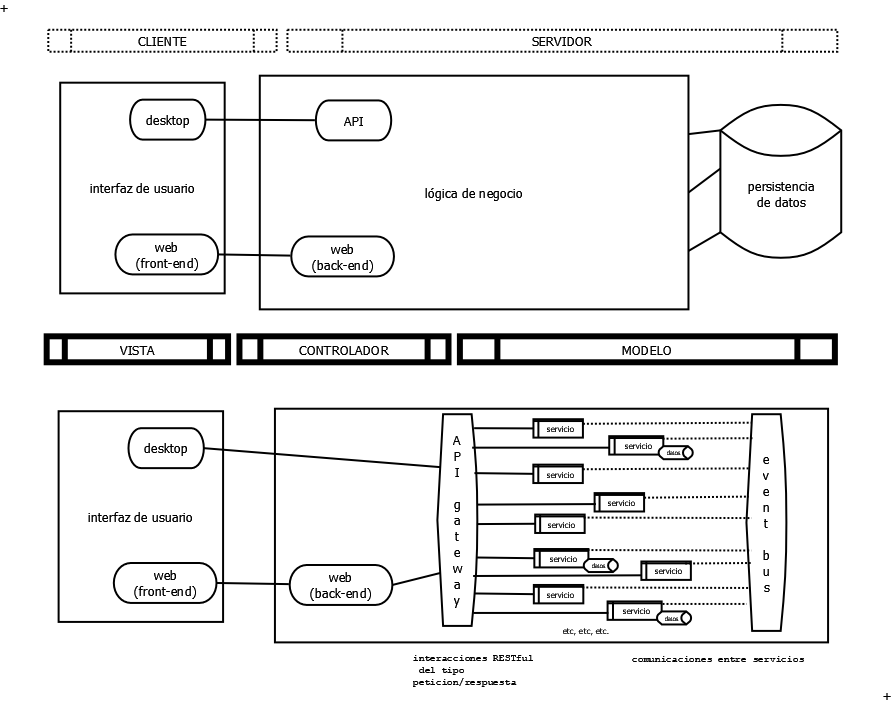
\includegraphics[width=1.1\textwidth]{arquitecturas multicapa}

El principal objetivo en cualquiera de estas arquitecturas multi-capa es desacoplar las capas entre sí.

Por ejemplo, separando:
\begin{itemize}
\item la forma de trabajar (medios de manipulación: ratón, teclado, gestos, voz,...) y de presentar información (gráfica, textual, auditiva,...),
\item del trabajo a realizar (información manejada y operaciones ejecutadas) 
\item de los datos a manipular (datos creados/leidos/modificados/borrados a través de esas operaciones) (nota: CRUD Create/Read/Update/Delete).
\end{itemize}

En una arquitectura multi-capa bien ejecutada, las capas tienen pocas dependencias (bajo acoplamiento) entre ellas. Y las dependencias están definidas de forma bien clara (`interfaces' concretos); con la intención de que las relaciones entre capas sean lo más estables posible.

Se facilita así la evolución del programa al permitir modificar capas concretas sabiendo de antemano cómo afectarán esos cambios a otras capas adyacentes.

De forma ideal, una arquitectura multi-capa bien ejecutada permite sustituir elementos en una de las capas sin afectar para nada a lo que hay en las otras capas, (o con mínimos cambios en alguna capa adyacente). 

Por ejemplo, debería ser posible sustituir sin demasiados problemas un interfaz gráfico basado en ventanas/ratón/teclado, por otro interfaz textual basado en comandos/parámetros, o por otro interfaz basado en servicios web {\footnotesize REST}. O por ejemplo, deberia ser posible sustituir una persistencia basada en archivos {\footnotesize XML}, por otra persistencia basada en archivos {\footnotesize JSON}, o por otra persistencia basada en una base de datos. O\ldots.

nota: No es que se vayan a realizar ninguna de esas sustituciones a lo largo de la vida útil del programa. El objetivo no es ese. Se trata de pensar en que se podrian realizar, para así ayudar a detectar dependencias y evitarlas.
\\Cuanto menos dependencias existan, más fácil será  comprender, mantener y evolucionar las distintas partes del programa. 

\vspace{1cm}

Una organización muy típica consiste en organizar el código en tres capas:
\begin{itemize}
\item MODELO: la parte que representa el dominio de la aplicación y que engloba la gestión de datos y la lógica de trabajo.
\item VISTA: la forma en que el modelo se muestra a los usuarios.
\item CONTROLADOR: la forma en que los usuarios interactuan con el modelo  a través de la vista.
\end{itemize}

El orden de las letras en el acrónimo MVC es importante. Se obtienen mejores resultados si primero se construye el modelo, luego la vista y, por último, el controlador. 
\\Aunque sin olvidar que todo proceso de construcción de software es iterativo y, por tanto, se irán realizando ajustes en el modelo, en la vista o en el controlador según se avanza en el trabajo en cualquiera de esas partes.

\begin{footnotesize}
notas:
\\Mientras se construye el modelo, para ejercitarlo y ver que funciona bien, se pueden utilizar test unitarios. No es necesario tener un interfaz de usuario (vista y controlador) para probarlo.
\\El modelo ha de recoger tanto la información (datos manejados) como el comportamiento (operaciones realizadas sobre esos datos). Un modelo que contemple solo datos se suele denominar ``modelo anémico''.
\\El controlador y la vista tienden a tener más acoplamiento entre sí. Es normal que sea así.
\\``Usuarios'' se ha de entender en sentido amplio, pudiendo ser tanto personas, como otros programas, como\ldots; es decir, es aquello que interactua con la aplicación desde ``el exterior'' de esta.
\end{footnotesize}

\begin{center}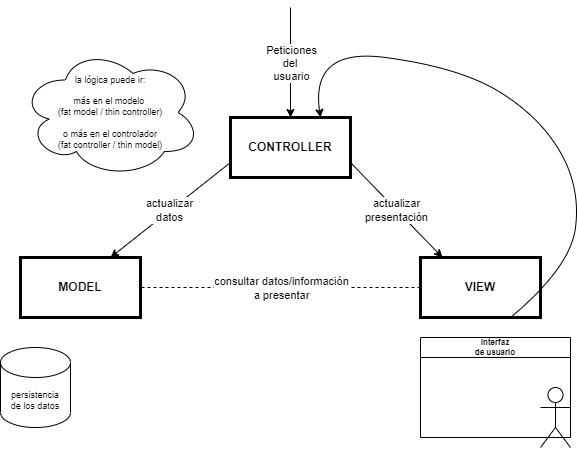
\includegraphics[width=0.7\textwidth]{division en capas - MVC}\end{center}

MVC puede tener varias interpretaciones, no todo el mundo lo interpreta igual:
\begin{center}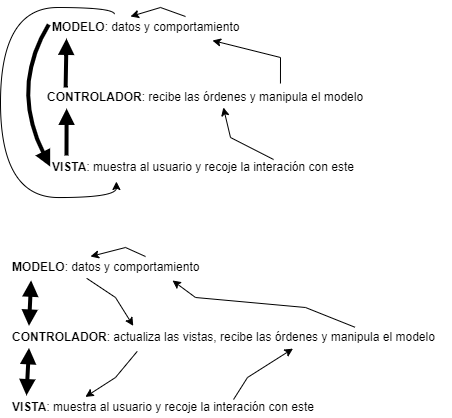
\includegraphics[width=0.7\textwidth]{division en capas - MVC - distintas interpretaciones}\end{center}

El patrón de arquitectura en tres capas también se conoce bajo otras denominaciones además de MVC ({\footnotesize Model-View-Controller}):  MVP ({\footnotesize Model-View-Presenter}), MVVM ({\footnotesize Model-View-ViewModel}), PMVC ({\footnotesize Persistence-Model-View-Controler}), etc.

Además, la idea puede ser extendida y ser aplicada en un sentido más amplio:
\begin{itemize}
\item ``MODELOs'': gestionan la información y los algoritmos de la aplicación.
\item ``CONTROLADORes'': hacen de adaptadores entre las vistas y los modelos.
\item ``VISTAs'': gestionan las peculiaridades tecnológicas de la interacción con el entorno exterior de la aplicación.
\end{itemize}
\begin{center}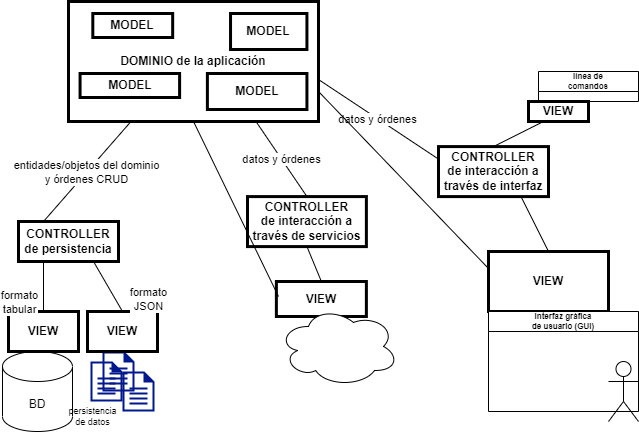
\includegraphics[width=0.8\textwidth]{division en capas - MVC -ampliada-}\end{center}

Al extenderla, quizá fuera mejor cambiarle el nombre de MVC ({\footnotesize Modelo-Vista-Controlador}) a MIAs ({\footnotesize Modelos-Infraestructuras-Adaptadores}):
\begin{itemize}

\item MODELOs: las funcionalidades, la parte que ``hace el trabajo'' , lo que es intrínseco a la resolución de las tareas relativas al dominio de aplicación.

\item INFRAESTRUCTURAs: las tecnologías usadas para que los modelos puedan realizar su trabajo. Por ejemplo: interfaz de usuario, persistencia en base de datos, interfaz con hardware específico, comunicaciones de red, servicios de terceros, etc.

\item ADAPTADOREs: los ``puentes'' que permiten a los modelos utilizar las infraestructuras sin quedar acoplados a ellas.

\end{itemize}

El orden en que se aborda el diseño/construcción del programa es el mismo que en MVC: primero se aborda el modelo, luego se aborda la infraestructura para hacerlo posible y, finalmente, se aborda el adaptador correspondiente para ligar ambos. 
\\De ahí que el orden de las letras sea similar: MIAs.
\\{\footnotesize nota: `vista' se equipara a `infraestructura' y `controlador' a `adaptador'.}

En el fondo, se persigue tener el mínimo de dependencias posibles entre los distintos elementos del programa. Y que estas dependencias queden lo más claras posibles.\footnote{Haciendo un símil con la confección de trajes, se suele hablar de tener claras las ``costuras'' entre las distintas partes.} Para permitir modificar/evolucionar cada parte concreta sin afectar a las demás.

Normalmente, serán los adaptadores los que dependan tanto de las infraestructuras(tecnologias) como de los modelos. Pero los modelos serán independientes de las infraestructuras(tecnologias). 

Siguiendo por ese camino, se puede llegar a la `arquitectura hexagonal' (también conocida como `ports and adapters').
\begin{center}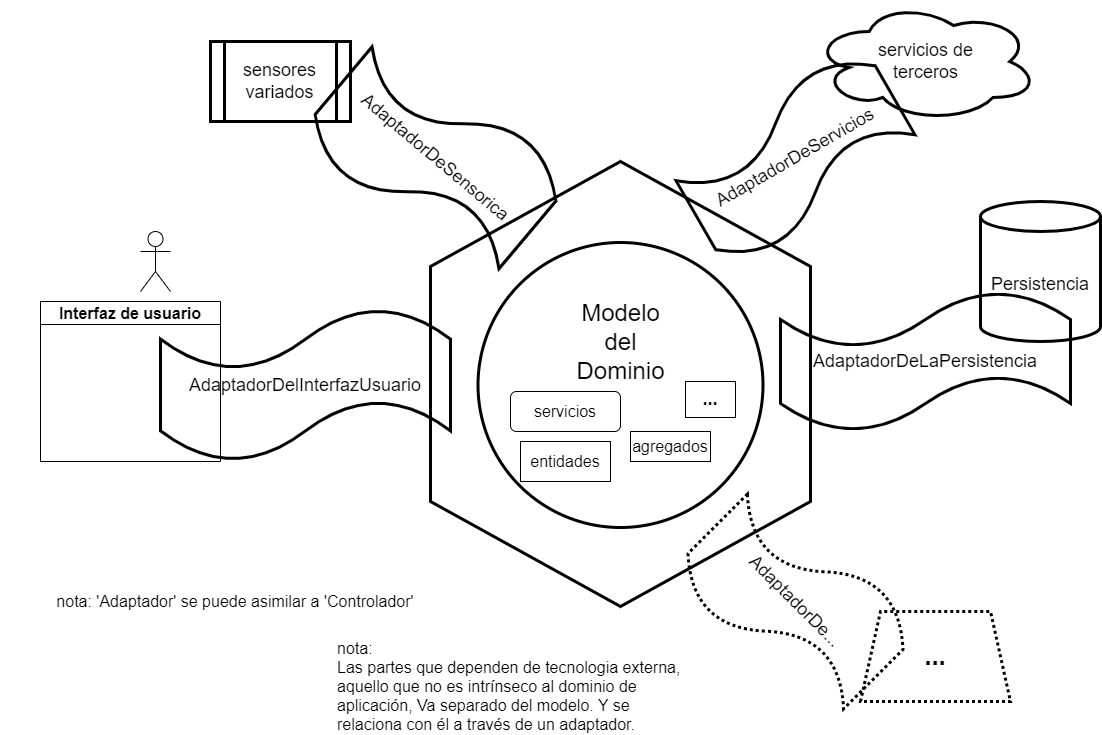
\includegraphics[width=0.8\textwidth]{Arquitectura Hexagonal}\end{center}




Pasando a otro tema. Una metodología muy práctica para guiar la organización del código en capas, sobre todo en softwares complejos, es la metodología \textbf{DDD} (Domain-Driven Design).

Un dominio es el contexto, entorno o disciplina donde se sitúa un determinado trabajo que se desea realizar. 

En la metodología DDD, se separan con claridad:
\begin{itemize}
\item Los aspectos intrínsecos funcionales relacionados con cada uno de los dominios del problema a resolver. 
\item Los aspectos tecnológicos incidentales relativos a la implementación de la solución con las herramientas concretas que se estén usando para ello.
\end{itemize}

\vspace{0.2cm}
Así, el programa resultante puede evolucionar de forma flexible. Según lo demande la parte de funcionalidades (dominio) o la parte tecnológica (infraestructura).

Pero DDD va mucho más allá de la separación en capas o en dominios. Contempla múltiples aspectos acerca de cómo encarar el diseño de un sistema software. 
\\(Eric Evans , \url{https://www.domainlanguage.com/ddd/})

Comenzando por el concepto primordial de `\textbf{ubiquitous language}': Todas las personas que participan en una determinada parte del sistema(un `bounded context'), han de hablar un lenguaje común. \footnote{En la documentación, en las reuniones,\ldots} Y ese lenguaje común consensuado se ha de ver reflejado también en el propio código. \footnote{En las denominaciones de variables, de funciones, de clases,\ldots}


\vspace{0.5cm}
La metodología DDD distingue diversos tipos de relaciones entre los diversos dominios que cohabitan dentro de un sistema.

Según cómo un dominio utilice o se sirva de otro, podemos tener:
\begin{itemize}

\item Colaboración (Parnership): ambas partes evolucionan de forma conjunta; teniendo en cuenta las necesidades de una y de otra.

\item Cliente-Servidor (Customer-Supplier): una parte proporciona servicios a la otra; y, en consecuencia, evoluciona teniendo en cuenta esa dependencia.

\item Conformismo (Conformist): una parte utiliza (tal cual) servicios de la otra; y, en consecuencia, se va adaptando (como pueda) a la evolución de esa otra.

\item Aislamiento (Anticorruption Layer): una parte utiliza servicios de la otra, pero lo hace a través de una capa de adaptación intermedia (proxy/adapter/facade); esto le proporciona una cierta independencia frente a la evolución de esa otra.

\end{itemize}

Según el grado de dependencia entre dominios, podemos tener:
\begin{itemize}

\item Independencia (Separate Ways): cada parte hace su trabajo tal cual, sin ninguna dependencia entre ellas; ambas pueden evolucionar cada una por su lado.

\item Coordinación (Open Host Service): las partes adoptan un protocolo de comunicación para coordinarse; mientras ambas respeten ese protocolo en sus interacciones, ambas pueden evolucionar cada una por su lado.

\item Compartición (Shared Kernel): las partes comparten una porción de modelo que sirve a ambas; cada una ha de mantener alineados sus respectivos conceptos internos relacionados con ese modelo común; pero, por lo demás, pueden evolucionar cada una por su lado.

\item Monolito (Big Ball of Mud):  no hay límites claros entre distintas responsabilidades y distintos dominios; las partes hacen un amplio uso directo unas de otras, según convenga; el sistema evoluciona ``como se pueda''\ldots
\\ {\footnotesize \url{http://laputan.org/mud/mud.html#Abstract}}

\end{itemize}


Las capas en un esquema DDD podrian encuadrarse en uno de estos tipos:
\begin{itemize}
\item MODELO De Dominio : (DOMAIN MODEL) : Recoge los ``entes'' propios del dominio. Recoge la ``lógica de negocio'' a nivel de cada uno de esos ``entes'' (cada uno contempla tanto la información que define su estado interno como las operaciones que admite para modificar dicho estado).
\item SERVICIOS De Dominio : (DOMAIN SERVICES) : Recoge la ``lógica de negocio'' a nivel de las operaciones que involucran a más de un ``ente'' del dominio o a una mezcla de ``entes'' y elementos externos al dominio.
\item ELEMENTOS AUXILIARES Comunes : (SHARED KERNEL) : Recoge aquellas partes de código comunes compartidas por varios dominios.
\item INFRAESTRUCTURA : (APPLICATION)(EXTERNAL WORLD) : Recoge los ``adaptadores'' empleados para que las  capas anteriores utilicen recursos externos (bases de datos, archivos, comunicaciones, periféricos,\ldots) o para que sean utilizadas desde el mundo exterior (interfaces de usuario, API pública,\ldots)
\end{itemize}

\begin{center}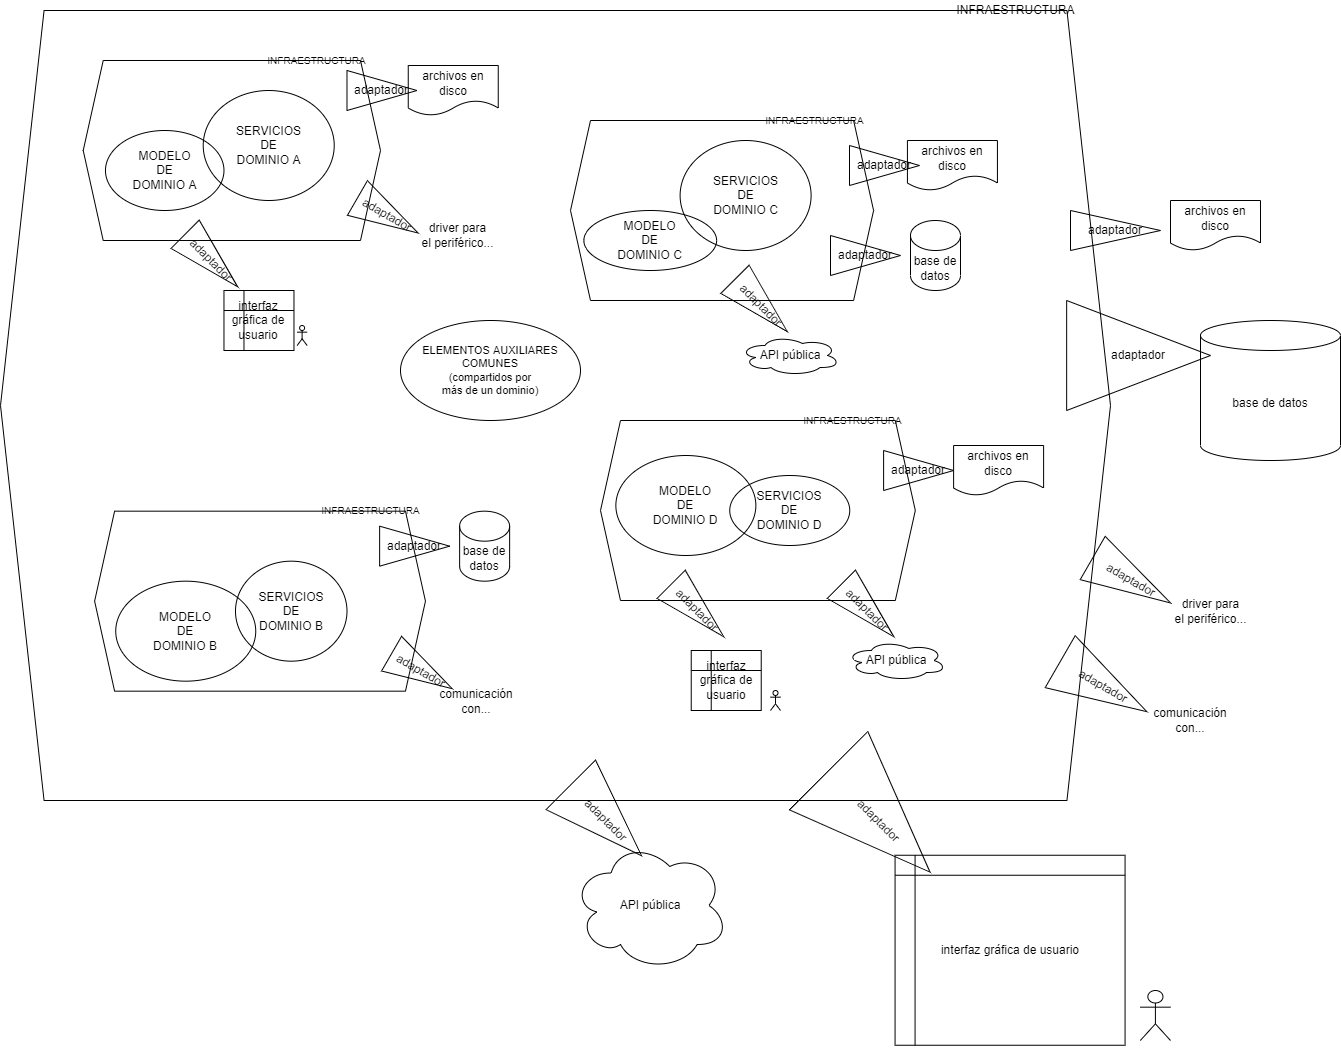
\includegraphics[width=0.9\textwidth]{division en capas - DDD}\end{center}


\begin{footnotesize}
Un ejemplo práctico de algunos de los conceptos citados puede verse en
\\ \url{https://github.com/JuanMuruaOlalde/Hotel}
\end{footnotesize}
\begin{scriptsize}
\\Aviso: está en construcción (y, por cierto, aún muy verde, solo empezando), así es que te animo a clonarlo y mirar de vez en cuando como va avanzando.
\end{scriptsize}

\begin{footnotesize}
Otro ejemplo práctico puede verse en \\ \url{https://github.com/JuanMuruaOlalde/DesarrolloDeSoftware/tree/main/02-Mas_alla_del_IF_y_del_WHILE/soluciones_java/MVC_springboot}
\end{footnotesize}

\begin{footnotesize}
Para complementar esta sección, puede resultar interesante informarse acerca de los \textbf{principios SOLID}. Por ejemplo, leyendo la correspondiente sección en el documento \url{https://www.susosise.es/documentos/Proyecto_Software.pdf}.
\end{footnotesize}


\section{Aplicaciones distribuidas} \label{AplicacionesDistribuidas}
Diversas aplicaciones (o procesos) corriendo de forma independiente en una misma máquina o en diversas máquinas. Cada aplicación realiza su trabajo, pero en algunos momentos colaboran entre ellas.

Para comunicarse entre sí, las diversas aplicaciones y servicios suelen seguir alguno de estos estilos de trabajo:
\begin{itemize}
\item Llamadas directas a procedimientos: (RCP, Remote Procedure Call). 
La aplicación que usa los servicios llama a estos a través de un trozo de código local (“proxy”) (“stub”) que tiene linkado en ella. Ese trozo local sabe cómo serializar/deserializar los datos (parámetros y respuestas) y sabe cómo llamar a las funciones en el otro trozo de código remoto (el servicio). El trozo remoto puede estar corriendo en la misma máquina o en otra cualquiera.
\\nota: cuando todas las llamadas son dentro de una misma máquina, se puede usar IPC (Inter-Process Communication), que es más directo; pero menos escalable (limitado a una sola máquina).

\item Llamadas asíncronas a recursos o servicios identificados con un URI (Universal Resource Identifier). La aplicación que usa los servicios llama a estos usando el URI correspondiente, normalmente usando el protocolo HTTP (\url{https://tools.ietf.org/html/rfc7231}). El servicio (recurso) identificado con esa URI le devuelve unos datos resultado, o le devuelve un archivo, o ejecuta una determinada acción concreta, o\ldots

\item Colas o tablones, de mensajes o de eventos: (MQ, Message Queue; EB, Event Bus o Event Broker; \ldots) 
La aplicación que usa los servicios deposita/envía mensajes a una cola. El servicio correspondiente recoge/recibe mensajes desde la cola, actúa en consecuencia y deposita/envía  (a la misma cola o a otra)  los correspondientes mensajes respuesta.
\\nota: Cuando la información intercambiada es más o menos sencilla o ``pasiva'' (solo representan estados, sucesos o envios de información), suelen denominarse eventos. Cuando esa información es más o menos compleja o ``activa'' (pueden representar órdenes, peticiones de servicio,\ldots; pueden requerir respuestas específicas; \ldots) suelen denominarse mensajes.
\\nota: Cuando es irrelevante el orden en que la información se deposita y en el que se lee, se suele denominar tablón. Cuando dicho orden es importante, se suele denominar cola.
\\nota:Las colas o tablones se suelen denominar también `temas' (topics) y cada una suele tener un propósito concreto y determinado.
\\La complejidad del sistema puede ir desde un simple publicar/subscribir, donde una parte deposita información y otras partes la leen. Hasta complejos protocolos de intercambios de mensajes/eventos para conseguir que dos o más procesos colaboren activamente entre sí, de forma asíncrona, para lograr llevar a cabo una tarea.

\end{itemize}

aviso: Una vez se comienza a trabajar en uno de esos estilos es muy difícil cambiar de estilo. Cuando se pone en marcha un proyecto grande basado en servicios, hay que sopesar cuidadosamente el balance entre los requisitos de sincronicidad, de tiempos de respuesta, de integridad transaccional y de escalabilidad. Para, en función de ello, decidir el estilo a emplear .



\vspace{1cm}
Algunas referencias ilustrativas:
\\ \url{https://www.mpich.org/}
\\ \url{https://computing.llnl.gov/tutorials/mpi/}
\\ \url{https://www.mpi-forum.org/docs/mpi-3.1/mpi31-report/mpi31-report.htm#Node0}



\section{Orientación a servicios \\ (SOA, SaaS, microservices,...) }
Se trata de encapsular cada una de las funcionalidades ofrecidas por el software, construyendo un servicio concreto para cada una de ellas. 

Un servicio se caracteriza porque recibe una cierta información al ser llamado (parámetros de petición) y devuelve una cierta información (una respuesta estructurada en un determinado formato).

Una aplicación se construye a base de realizar llamadas a los servicios disponibles.

En los sistemas más sofisticados, suele haber algún mecanismo (un catálogo) para que las aplicaciones puedan ``consultar'' los servicios disponibles en el sistema y ``aprender'' cómo se utiliza cada uno.



\section{Orientación a servicios, arquitectura REST \\(REpresentational State Transfer)}

REST no es un estandard ``per se'', sino una forma de trabajar. Son una serie de restricciones que nos autoimponemos en la arquitectura de nuestra aplicación. Para conseguir un software ``bien adaptado a la web'' (a la nube), uno que sea fácilmente escalable ``a escalas Internet'' (planetarias).

Básicamente se trata de:

\begin{itemize}

\item Ser cliente-servidor: la parte cliente (frontend) se encarga de interactuar con el usuario y la parte servidor (backend) se encarga de manipular la información (los recursos).

\item Permitir poner intermediarios entre la parte cliente y la parte servidor. Siendo estos transparentes para la funcionalidad.
\\{\footnotesize Por ejemplo: balanceadores de carga, cachés de información \footnote{Para poder ser cacheada, cada porción de información (cada recurso) ha de establecer con claridad si un intermediario puede o no guardarsela para reutilizarla cuantas veces la necesite, sin volver a solicitarla al servidor.}, sistemas de seguridad, etc.}

\item Prescindir de la necesidad de tener en cuenta estados internos de la aplicación (ser ``stateless''). Cada llamada a un servicio o acción (a un ``endpoint'') es independiente. No depende de las llamadas previas a ese mismo o a otros servicios o acciones.

{\footnotesize nota: Es conveniente que también sea idempotente, que una misma llamada  pueda llegar repetida varias veces al servidor o al cliente sin causar efectos extraños ni duplicidades no deseadas.}

\item Permitir personalización bajo demanda. El cliente puede recibir actualizaciones desde el servidor para ampliar o modificar la funcionalidad del sistema.

\item Tener un interfaz uniforme para todos los ``endpoint'' (servicios o acciones) involucrados:

\begin{itemize}

\item Todos los recursos afectados en cada llamada se identifican con claridad y sin ambigüedades. 
\\{\footnotesize (Por ejemplo, utilizando URIs o IDs o UUIDs o\ldots)}

\item Los recursos se manipulan a través de una representación de los mismos. Dicha representación contiene en sí misma todo lo que un cliente necesita saber para poder consultarlos, crearlos, modificarlos o eliminarlos.
\\{\footnotesize (Por ejemplo siguiendo los estandares de comandos de HTTP: GET, POST, PUT, PATCH, DELETE,\ldots)}

\item Toda la información intercambiada, en todos los mensajes, es autodescriptiva. Cada mensaje contiene todo lo necesario para que su receptor sepa cómo ha de ha de tratarlo.
\\{\footnotesize (Por ejemplo, utilizando identificadores MIME y formatos textuales fácilmente reconocibles, tales como HTML, XML, JSON,\ldots)}

\item La navegación por las diversas etapas o estados de la aplicación se realiza a través de hipervínculos. Cada paso guía al cliente hacia los siguientes pasos disponibles a partir de ahí.
\\(HATEOAS, Hypermedia as the Engine of Application State)
\\En cierta manera, se podria decir que para utilizar bien una buena API\footnote{API: exponer la lógica de un software (servidor) para poder ser consumida o utilizada por otros softwares (clientes)} REST no se necesitaría consultar instrucciones prefijadas de antemano.
Bastaría conocer el punto de inicio (la primera URL a la que llamar). Y, a partir de ahí, se continuará a base de ir leyendo e interpretando la información intercambiada en cada paso.
\\{\footnotesize (Por ejemplo, usando documentos HAL: JSON Hypertext Application Language)}
\end{itemize}

\end{itemize}

\vspace{0.5cm}
Un enlace ilustrativo:
\\ \url{https://martinfowler.com/articles/richardsonMaturityModel.html}


\vspace{1cm}
nota: 
\\Habitualmente, las APIs REST se suelen implementar usando HTTP como protocolo de transporte/interacción y JSON como formato de estructuración de la información. 
\\Pero también podrían ser implementadas de otras formas. Utilizando cualquier otro formato textual legible por personas humanas y cualquier otra combinación de protocolos estándares habituales en el campo de aplicación donde se esté trabajando.

\vspace{1cm}
nota: 
\\La persona que acuñó el término REST, Roy Fielding, ha comentado en más de una ocasión que la caracteristica principal para ser `RESTful' es la organización de la navegación dentro de las aplicaciones utilizando hipervínculos (HATEOAS). Pero, en la práctica, casi ninguna de las implementaciones de REST hace uso de la misma. Ni en la parte servidora. Ni, mucho menos, en la parte cliente. Temas como los documentos HAL no han terminado de cuajar en la práctica\ldots


\section{Ejercicios}

\url{https://github.com/JuanMuruaOlalde/sugerencias-para-practicar-programacion/tree/main/Multiinterface}

\url{https://github.com/JuanMuruaOlalde/sugerencias-para-practicar-programacion/tree/main/MVC}

\url{https://github.com/JuanMuruaOlalde/sugerencias-para-practicar-programacion/tree/main/Excursiones}

\url{https://github.com/JuanMuruaOlalde/Albaranes}

\url{https://github.com/JuanMuruaOlalde/sugerencias-para-practicar-programacion/tree/main/Hotel}




\chapter{apéndice A: ejemplos de posibles herramientas de trabajo}
Este es un compendio de mis herramientas favoritas a día de hoy (Julio 2020). Que quede claro que hay muchas otras disponibles y que cada cual es libre de utilizar las que prefiera.

nota: Todas las herramientas citadas, o bien son directamente software libre o bien tienen una versión de uso libre (Community Edition).

\section{Para programar en Java}
Un compilador-debugger ::: JDK (Java Development Kit), por ejemplo:
\\ \url{https://adoptium.net/es/}
\\ (o OpenJDK: \url{https://jdk.java.net})
\\ (o el JDK comercial de Oracle: \url{https://www.oracle.com/java/technologies/javase-downloads.html})

Un IDE ::: Eclipse: \url{https://www.eclipse.org}
\\(o Netbeans: \url{https://netbeans.apache.org})
\\(o IntelliJ IDEA: \url{https://www.jetbrains.com/es-es/idea})
\\etc.

Un entorno de pruebas unitarias ::: JUnit: \url{https://junit.org}

Un entorno de registro de eventos ::: JLog: \url{https://logging.apache.org/log4j}

Una biblioteca GUI ::: incluidas en la plataforma: \textit{java.awt, java.swing} (ambas ya ``deprecated''?). \begin{footnotesize}(Nota: para facilitar los primeros pasos con \begin{scriptsize}AWT\end{scriptsize} y Swing puede ser útil un complemento tal como WindowBuilder: \url{https://www.eclipse.org/windowbuilder}.)\end{footnotesize} 
\\ Otra biblioteca también incluida en la plataforma: \textit{JavaFX} ( la que se recomienda usar hoy en día). Es algo más compleja, pero permite implementar interfaces de usuario mucho más ricos.  \begin{footnotesize}(Nota: para facilitar los primeros pasos, puede ser útil un complemento tal como JavaFX Scene Builder: \url{https://gluonhq.com/products/scene-builder/})\end{footnotesize} 

Un parser XML ::: (incluido en la plataforma: javax.xml)

Interactuar con una base de datos ::: (biblioteca incluida en la plataforma: \begin{footnotesize}JDBC:\end{footnotesize}  \textit{java.sql , javax.sql}) \begin{footnotesize} Nota: el uso de esta biblioteca requiere del correspondiente driver JDBC para el motor de base de datos utilizado. Por ejemplo \url{https://jdbc.postgresql.org/} o \url{https://dev.mysql.com/doc/connectors/en/connector-j-usagenotes-basic.html}\end{footnotesize}

Un analizador estático de código 
\\::: Maven PMD Plugin: \url{https://maven.apache.org/plugins/maven-pmd-plugin} 
\\::: SonarLint \url{https://www.sonarlint.org/}

\begin{footnotesize}
(Nota: El uso de Maven -o de su sucesor Gradle-, con sus variados plugins para todo el ciclo de desarrollo, puede ser una buena forma de introducirse en el mundo de la integración/despliegue continuos (CI/CD).)
\end{footnotesize}

Un analizador de rendimiento (profiler) ::: No he encontrado uno de licencia libre que me llamara la atención; algunos comerciales pueden ser: 
\\YourKit: \url{https://www.yourkit.com}  
\\JProfiler: \url{https://www.ej-technologies.com/products/jprofiler/overview.html}

\section{Para programar en C++}

Un IDE ::: QT Creator: \url{https://www.qt.io/developers}  

Un compilador-debugger ::: (incluido en la plataforma: gcc/g++)

Un entorno de pruebas unitarias ::: (incluido en la plataforma: QTest)

Un entorno de registro de eventos ::: (incluido en la plataforma: QMessageLogger)

Una biblioteca GUI ::: (incluida en la plataforma: QWidgets --interfaces estáticos--) (también incluida en la plataforma: QML/QtQuick --algo más compleja; pero permite implementar interfaces de usuario mucho más dinámicos--)

Un parser XML ::: (incluido en la plataforma: QXml)

Interactuar con una base de datos ::: (incluido en la plataforma: QPSQL) 

Un analizador estático de código ::: (incluido en la plataforma: Clang Tools)

Un analizador de rendimiento (profiler) ::: Valgrind: \url{https://www.valgrind.org} 

\section{Para programar en C\#}

Un IDE ::: Visual Studio: \url{https://visualstudio.microsoft.com/es/vs/community/} 

Un compilador-debugger ::: (incluido en la plataforma)

Un entorno de pruebas unitarias :::  (incluido en la plataforma)

Un entorno de registro de eventos ::: (incluido en la plataforma: \textit{System.Diagnostics})
\\o Nlog (paquete nuget)
\\o Log4net: \url{https://logging.apache.org/log4net}

Una biblioteca GUI ::: (incluida en la plataforma: \textit{Forms} --interfaces estáticos--) o (también incluida en la plataforma: \textit{WPF} --algo más compleja; pero permite implementar interfaces de usuario mucho más dinámicos--) 

Un parser XML ::: (incluido en la plataforma: \textit{System.Xml})

Interactuar con una base de datos ::: (biblioteca incluida en la plataforma: \begin{footnotesize}ADO.NET:\end{footnotesize} \textit{ System.Data}) \begin{footnotesize}Nota: el uso de esta biblioteca requiere del correspondiente conector para el motor de base de datos utilizado. Por ejemplo \url{https://www.npgsql.org/} o \url{https://dev.mysql.com/doc/connector-net/en/connector-net-introduction.html})\end{footnotesize} 

Un analizador estático de código :::   (incluido en la plataforma)

Un analizador de rendimiento (profiler) :::   (incluido en la plataforma)


\section{Para programar en Python}

Un intérprete-debugger ::: Python: \url{https://www.python.org} 

Un IDE ::: Eclipse: \url{https://www.eclipse.org} 
\\con el complemento PyDev: \url{https://www.pydev.org} 

Un entorno de pruebas unitarias ::: (incluido en la plataforma)\url{https://docs.python.org/3/library/unittest.html}

Un entorno de registro de eventos ::: (incluido en la plataforma)\url{https://docs.python.org/3/library/logging.html}

Una biblioteca GUI ::: (incluida en la plataforma)\url{https://docs.python.org/3/library/tk.html}
\\(También hay otras ::: \url{https://docs.python.org/3/library/othergui.html})

Un parser XML ::: (incluido en la plataforma)\url{https://docs.python.org/3/library/xml.html}

Interactuar con una base de datos ::: Psycopg: \url{https://www.psycopg.org} 

Un analizador estático de código ::: PyLint: \url{https://www.pylint.org} 

Un analizador de rendimiento (profiler) ::: PyVmMonitor: \url{https://www.pyvmmonitor.com} 

nota: Python es un lenguaje interactivo que se está usando cada vez más en ámbitos científicos. En esos ámbitos se suele utilizar en forma de ``cuaderno'', en vez de dentro de un `entorno de programación profesional'. Estos cuadernos pueden ser una buena manera de comenzar a trabajar con Python.
\\ \url{https://jupyter.org/}
\\ \url{https://github.com/jupyterlab/debugger}
\\ \begin{footnotesize}\url{https://blog.jupyter.org/a-visual-debugger-for-jupyter-914e61716559}\end{footnotesize}
\\nota: Entre otros proveedores de ese servicio, Google es uno de los que permite trabajar con cuadernos Jupyter online. En su plataforma Google Colab \url{https://colab.research.google.com/notebooks/intro.ipynb}

\section{Para programar en HTML5/CSS/Javascript}

Los tres componentes base:
\begin{itemize}
\item HTML: organiza el contenido de las páginas mostradas al usuario (frontend).
\item CSS: organiza la presentación, la apariencia de esas páginas.
\item Javascript: es el lenguaje de programación para el que prácticamente todos los navegadores web tienen soporte.
\\{\footnotesize nota: en la parte del servidor web (backend), además de Javascript, se pueden emplear también otros lenguajes de programación: Python, Typescript, Java, C\#, PHP, Ruby, Go,\ldots}
\end{itemize}

El interface gráfico de usuario ::: páginas HTML/CSS/javascript estandar
\\::: MDN \url{https://developer.mozilla.org/en-US/docs/Web}
\\W3Consortium \url{https://www.w3.org/standards/webdesign/}

Complementadas con alguna biblioteca javascript auxiliar para facilitar el trabajo y conseguir interfaces más ricos. Por ejemplo:
\\::: Bootstrap.js \url{https://getbootstrap.com/}
\\::: Angular.js \url{https://angularjs.org/}
\\::: React.js \url{https://reactjs.org/}
\\::: Vue.js \url{https://vuejs.org/}
\\::: \url{https://openjsf.org/projects/}
\\::: etc, etc,

Un intérprete-debugger ::: los propios navegadores web suelen incluir  herramientas para inspeccionar el código de las páginas visualizadas. (clic-dcho, 'Inspeccionar' o la tecla [F12] o\ldots)

Una herramienta interesante ::: \url{https://www.browsersync.io} (Es un pequeño servidor web en sí mismo o un complemento de otro servidor web mayor. Permite actualizar rápidamente el contenido servido, facilitando así la prueba local de páginas según se van desarrollando.)

Para aplicaciones ``grandes'' se hace necesario contar con un servidor web ``de producción'' tal como, por ejemplo:
\\::: Apache \url{https://httpd.apache.org}
\\::: Nginx \url{https://nginx.org} 
\\Estos servidores suelen proporcionar la plataforma necesaria para generar de forma dinámica las páginas web y para ejecutar aplicaciones de lógica y datos que las soporten. 


En lugar de disponer de nuestros propios servidores (``on-premise'') y la infraestructura asociada a ellos, también es posible recurrir a los servicios de plataforma de alguien externo (``en la nube''), como por ejemplo:
\\ \url{https://cloud.google.com/}
\\ \url{https://aws.amazon.com/es/}
\\ \url{https://azure.microsoft.com/es-es/}
\\ \url{https://www.digitalocean.com/}
\\ \url{https://www.heroku.com/home}
\\ etc, etc, (cada vez hay más y más oferta de plataformas ``cloud'')


\section{Una herramienta transversal: almacenamiento de código con control de versiones}

\textbf{Git}: \url{https://git-scm.com}
\\complementado con un interfaz gráfico para hacer más claro y sencillo el trabajo, 
\textbf{Sourcetree}: \url{https://www.atlassian.com/software/sourcetree} 

nota: Si se va a trabajar entre varias personas, y sobre todo si estas trabajan desde ubicaciones diferentes. Se necesita contar también con un almacenamiento central compartido. Por ejemplo, en la nube, \textbf{Bitbucket}: \url{https://www.atlassian.com/software/bitbucket} 

\section{Otra herramienta transversal: motor de base de datos}
PostgreSQL: \url{https://www.postgresql.org}
\\o\\
MariaDB: \url{https://mariadb.org/}





\end{document}
